\documentclass[lettersize,journal]{IEEEtran}

% *** CITATION PACKAGES ***
\usepackage{cite}
\usepackage{graphicx}
\usepackage{enumitem}
\usepackage{listings}
\usepackage{subcaption}
\usepackage{amsmath,amssymb} 
\usepackage{algorithm, algpseudocode}
% \renewcommand*{\figureautorefname}{Fig.} 
\graphicspath{{figures/}}
\DeclareGraphicsExtensions{.jpg}

%\usepackage[caption=false,font=footnotesize]{subfig} 


% *** PDF, URL AND HYPERLINK PACKAGES ***
\usepackage{hyperref}  
\hypersetup{
    colorlinks=true,
    linkcolor=blue,    
    urlcolor=cyan, 
}


\begin{document}

\title{Lab 3 - Hough Transform \\ \vspace{0.1em} \LARGE Computational Vision \& Imaging}

\author{\textbf{Student ID}: XXXXXXX \\
~\IEEEmembership{Random Student,~School of Computer Science,\\University of Birmingham, UK, B15 2TT}
% <-this % stops a space
\thanks{This is a solution for the Formative Assignment by Hamid Dehghani}
% <-this % stops a space
\thanks{The report was submitted to Canvas on Mar 04 and reviewed by a TA}}

% The paper headers
\markboth{Collection of Lab Reports, Computer Vision, No.~3, March~2022}%
{Shell \MakeLowercase{\textit{et al.}}: A collection of Report submissions documenting assignment solutions}

\maketitle

\begin{abstract}
This document is a formal solution for the Lab 3 Formative Assignment based on Hough Transform. It analyses the algorithm of detecting lines in the image using Hough Transform. It checks the impact of changing the number of desired lines to detects and experiments with different edge filters required to produce an input for the Hough Transform.
\end{abstract}

\begin{IEEEkeywords}
Lab 3, formative assignment, computer vision, imaging, Hough Transform, filters, kernels, Roberts, Prewitt, Sobel, Laplacian, Gaussian, Canny, MATLAB.
\end{IEEEkeywords}

\section{Introduction}
\IEEEPARstart{B}{uilding} on top of the previous topics \emph{Edge Detection} and \emph{Noise Removal}, we were introduced to another important task in imaging - \emph{line detection}. After having the edges of the image, they can be used to determine and match with the straight lines. The method this paper analyses is \textbf{Hough Transform}. Detecting line segments is an important feature in machine vision.

\section{Setup}
We continue the setup of the first 2 labs because the methods for edge detection, such as \emph{Sobel} or \emph{Laplacian} operators will be reused here. One additional operator, not covered before but that is going to be used in the experiments is \textbf{Prewitt}. It works the same way as the \emph{Sobel} operator and its horizontal and vertical filters can be seen in \autoref{eq:1}. 

\begin{equation}\label{eq:1}
    G_X = \begin{bmatrix}-1 & 0 & 1 \\ -1 & 0 & 1 \\ -1 & 0 & 1\end{bmatrix};\ 
    G_Y = \begin{bmatrix}-1 & -1 & -1 \\ 0 & 0 & 0 \\ 1 & 1 & 1\end{bmatrix}
\end{equation}

This time we're given a different image "cluttera2.jpg" which can be seen in \autoref{fig:1}.

\begin{figure}[h]
    \centering
    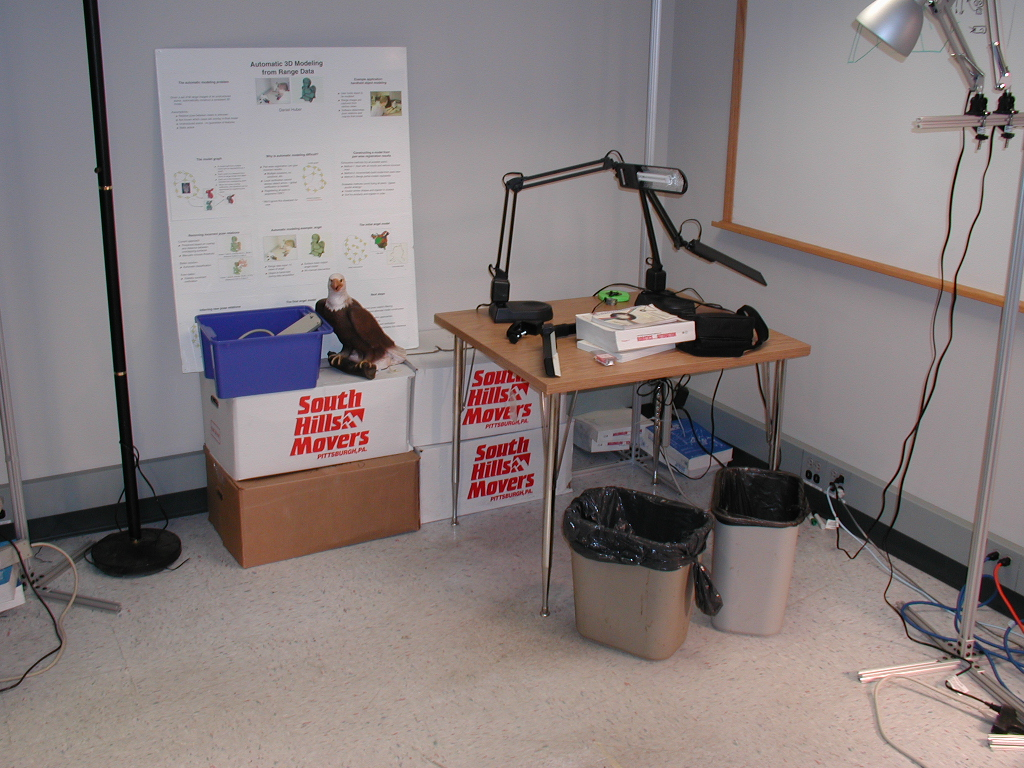
\includegraphics[width=0.55\linewidth]{cluttera2}
    \caption{Cluttera}
    \label{fig:1}
\end{figure}

\section{Methodology}

Before \autoref{section:4}, it is necessary to explain certain algorithms met while completing the tasks - \textbf{Canny Edge Detection} and \textbf{Hough Transform}.

\subsection{Canny Edge Detection}

It is a relatively straightforward algorithm considering Canny's observation that the first derivative of the \emph{Gaussian} provides an operator that optimizes signal-to-noise ratio and localisation \cite{ref1}. The algorithm works like this:

\hfill

\begin{enumerate}
    \item Compute the image gradients $\nabla_x f = f * \nabla_x G$ and $\nabla_y f = f *\nabla_y G$ where $G$ is the \emph{Gaussian} function of which the kernels can be found by:
    \begin{itemize}
        \item $\nabla_x G(x, y)=-\frac{x}{\sigma^2}G(x, y)$
        \item $\nabla_y G(x, y)=-\frac{y}{\sigma^2}G(x, y)$
    \end{itemize}
    \item Compute image gradient \emph{magnitude} and \emph{direction}
    \item Apply \textbf{non-maxima} suppression
    \item Apply \textbf{hysteresis} thresholding
\end{enumerate}

\hfill

\noindent\textbf{Non-maxima suppression} - checking if gradient magnitude at a pixel location along the gradient direction (\emph{edge normal}) is local maximum and setting to ` if it is not

\hfill

\noindent\textbf{Hysteresis thresholding} - a method that uses 2 threshold values, one for certain edges and one for certain non-edges (usually $t_h = 2t_l$). Any value that falls in between is considered as an edge if neighboring pixels are a strong edge.

\subsection{Hough Transform}

We know that a point in \emph{Cartesian space} can represented in \emph{Polar space} as a point from the origin at some angle as can be seen in \autoref{eq:2}.

\begin{equation}\label{eq:2}
    \rho = x \cos \theta + y \sin \theta
\end{equation}

When talking about \textbf{Hough Transform} we are concerned with parameters (explained below) and by using this \emph{Polar} representation, we impose limits for the parameters - $\theta\in[-90, 90)$ and $\rho\in[0, \text{image diagonal}]$ - and so they can't go to infinity. We want to find the parameters that describe a line and for this we introduce \textbf{Hough Space}.

\hfill

\noindent\textbf{Hough Space} - a plane defined by $\rho$ and $\theta$ which takes points $(x, y)$ in image space and represents them as sinusoids in the new space. Each point in such space $(\rho, \theta)$ is parameters for a line in the image space.

\hfill

To perform \textbf{Hough Transform}, we take the mostly intersected points of sinusoids in the \textbf{Hough Space} and map them back to the lines in the image space. Such lines pass through those points which as sinusoids were part of the intersection point. The process can be seen in algorithm \ref{alg:1}.

\begin{algorithm}
    \caption{Hough Transform}\label{alg:1}
    \begin{algorithmic}
        \State Initialize vectors $\boldsymbol{\rho}$ and $\boldsymbol{\theta}$ for all possible lines
        \State Initialize matrix $A$ of zeros indexed by $\rho_i$ and $\theta_j$
        \For {each point $(x, y)$}
            \For {each angle $\theta$}
                \State $\rho \gets x \cos \theta + y \sin \theta$
                \State $A[\rho, \theta] \gets A[\rho, \theta] + 1$
            \EndFor
        \EndFor
        \State where $A > \text{Threshold}$ return a line
    \end{algorithmic}
\end{algorithm}

We also still need to suppress non-local maxima. Note that there are generalised versions for ellipses, circles etc. But we are concerned with a line equation, i.e., MATLAB works with \textbf{Standard Hough Transform}.

\section{Tasks}\label{section:4}
\subsection{Task 1}

\noindent Task 1 asks to walk through the script file and explain how each function works, from edge detection, \emph{Hough Transform} to line detection. The answer is presented in the following paragraphs.

\hfill

\noindent\textbf{Edge Detection}

Firstly, the algorithm takes an image, converts it to greyscale and applies \emph{Canny Edge Detection} technique to identify borders. It applies \emph{Gaussian filter} derivative to compute image gradients, computes their magnitude, applies \emph{Non-maxima Suppression} and \emph{Hysteresis Thresholding}. The output is a binary image matrix with pixels with values of 1 indicating edges. The output edge map of the given image can be seen in \autoref{fig:2}.

\begin{figure}[h]
    \centering
    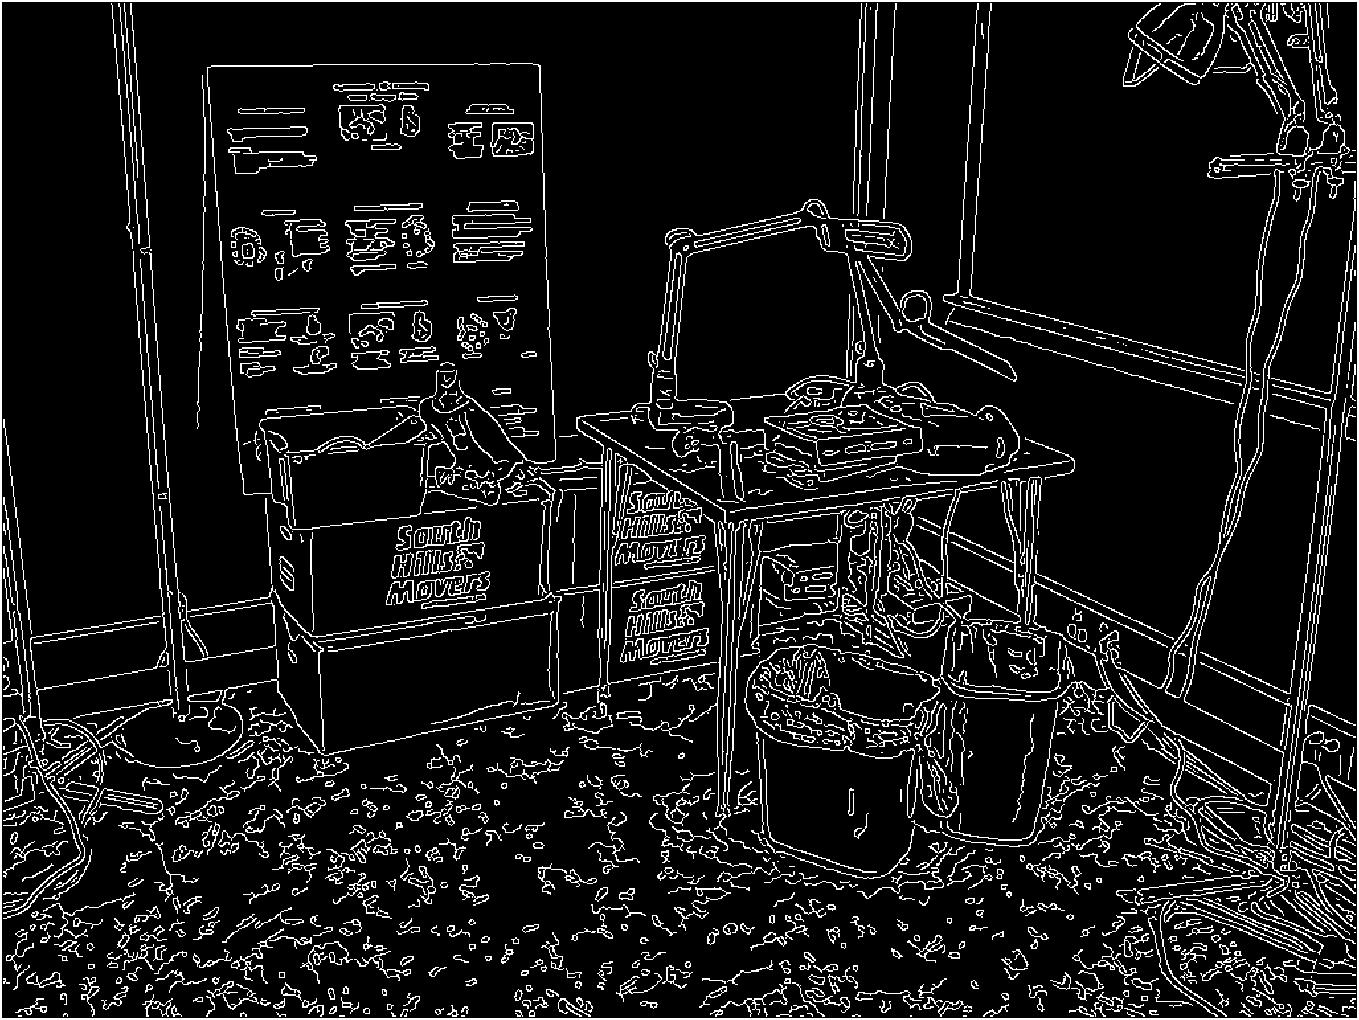
\includegraphics[width=0.8\linewidth]{edge_map_canny}
    \caption{Cluttera edge map}
    \label{fig:2}
\end{figure}

The explanation corresponds to MATLAB documentation: \emph{"The Canny method finds edges by looking for local maxima of the gradient of I. The gradient is calculated using the derivative of a Gaussian filter. The method uses two thresholds, to detect strong and weak edges, and includes the weak edges in the output only if they are connected to strong edges. This method is therefore less likely than the others to be "fooled" by noise, and more likely to detect true weak edges."}

Note that the threshold values are determined automatically and the default sigma value is $\sqrt 2$

\hfill

\noindent\textbf{Hough Transform}

Secondly, the algorithm applies \emph{Standard Hough Transform}, where it takes a binary image matrix and transforms image space to \emph{Hough} space (maps points to sinusoids). It digitalizes each line to a parameter matrix where each entry is incremented if a discrete line passes through that matrix cell. The output is the matrix itself with rows representing possible magnitudes and columns representing all possible angles. It also returns an array of considered angles and an array of considered magnitudes.

The explanation corresponds to MATLAB documentation: \emph{"hough(BW) computes the Standard Hough Transform (SHT) of the binary image BW. The hough function is designed to detect lines. The function uses the parametric representation of a line: rho = x*cos(theta) + y*sin(theta)."}

\hfill

Thirdly, the algorithm finds \emph{Hough Peaks} - it takes the \emph{Hough Transform} matrix and finds up to specified number of peaks (in the provided case, up to 10), whithin a specific minimum threshold (in the provided case, 0.3 times the maximum value of the \emph{Hough} matrix). The output is a coordinate matrix with rows representing coordinates of the peaks in the parameter matrix. Visualized \emph{Hough Transform} with identified peaks of the provided image can be seen in \ref{fig:3}.

\begin{figure}[h]
    \centering
    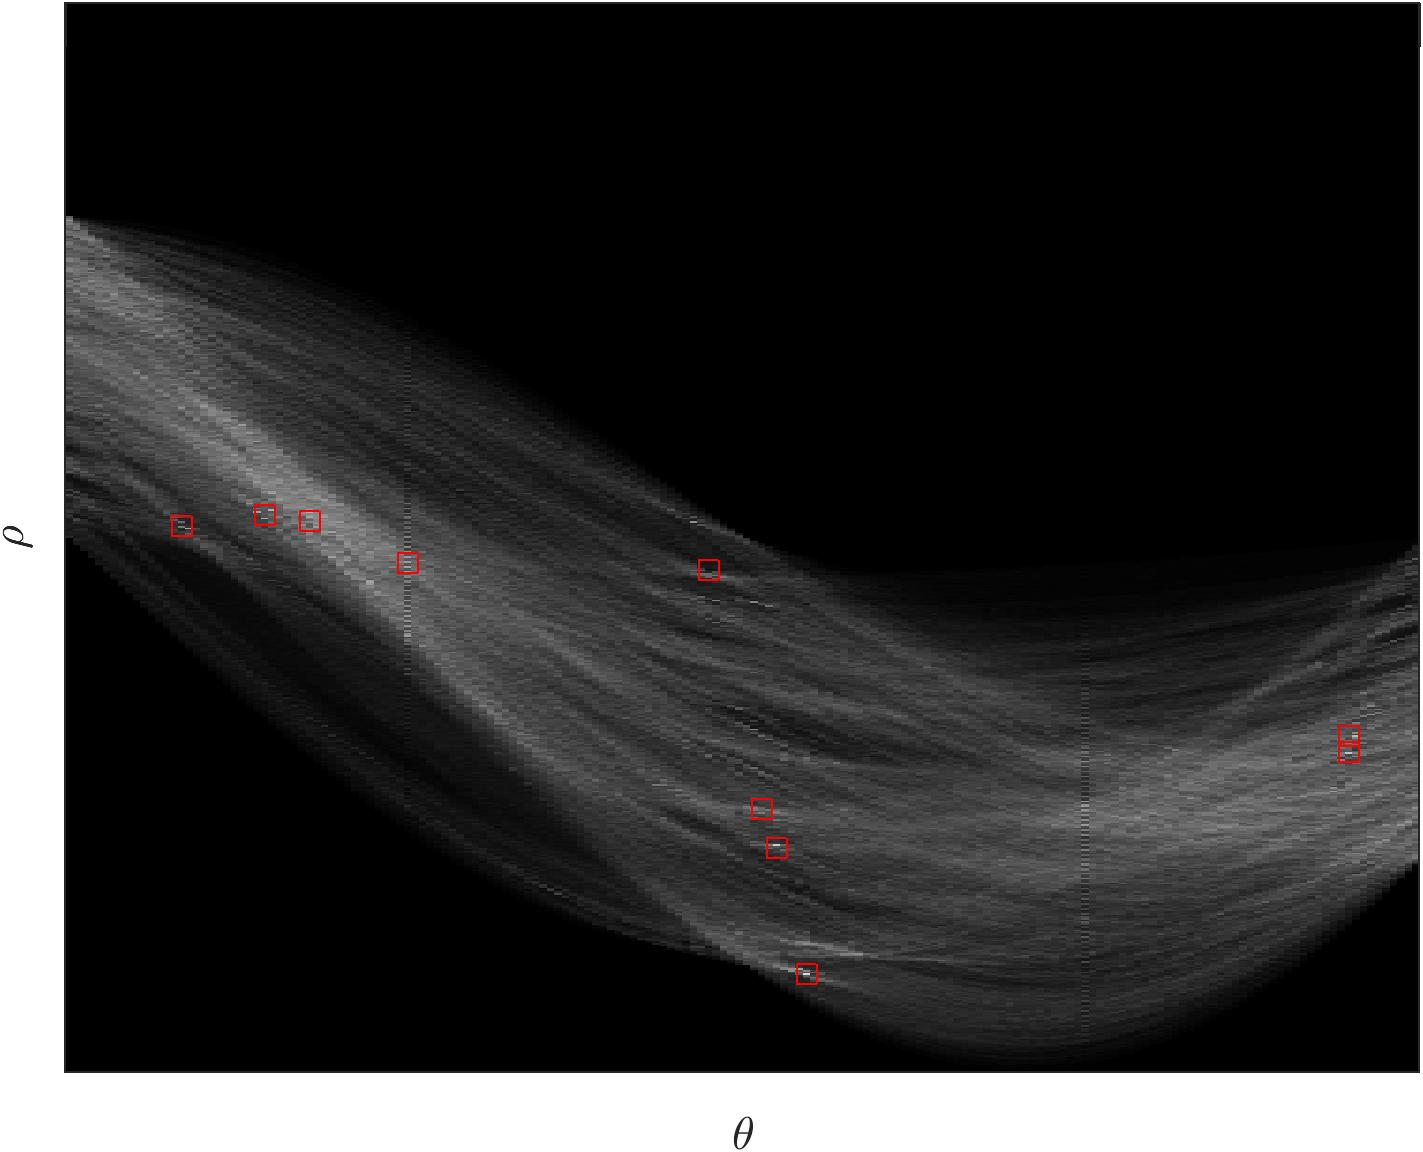
\includegraphics[width=0.8\linewidth]{hough_transform_10}
    \caption{Cluttera Hough Transform}
    \label{fig:3}
\end{figure}

The explanation corresponds to MATLAB documentation: \emph{"houghpeaks(H,numpeaks) locates peaks in the Hough transform matrix, H, generated by the hough function. numpeaks specifies the maximum number of peaks to identify."}

\newpage

\noindent\textbf{Line Detection}

Finally, the line segments are extracted via `houghlines` method. It takes in the \emph{Hough} matrix, theta and rho values as well as calculated peaks and computes the line segments in the image. A threshold to merge multiple lines to one (in the provided case, 5) and a minimum line length (in the provided case, 7) can also be specified. The start and the finish of the line is determined by checking the original edge values to check whether there actually should be a line. Idea of edge connectivity is used through named parameter 'FillGap' which is a distance between 2 line segments of the same bin. \emph{"When the distance between the line segments is less than the value specified, the houghlines function merges the line segments into a single line segment".} The output with line segments of the provided image can be seen in \autoref{fig:4}.

\begin{figure}[h]
    \centering
    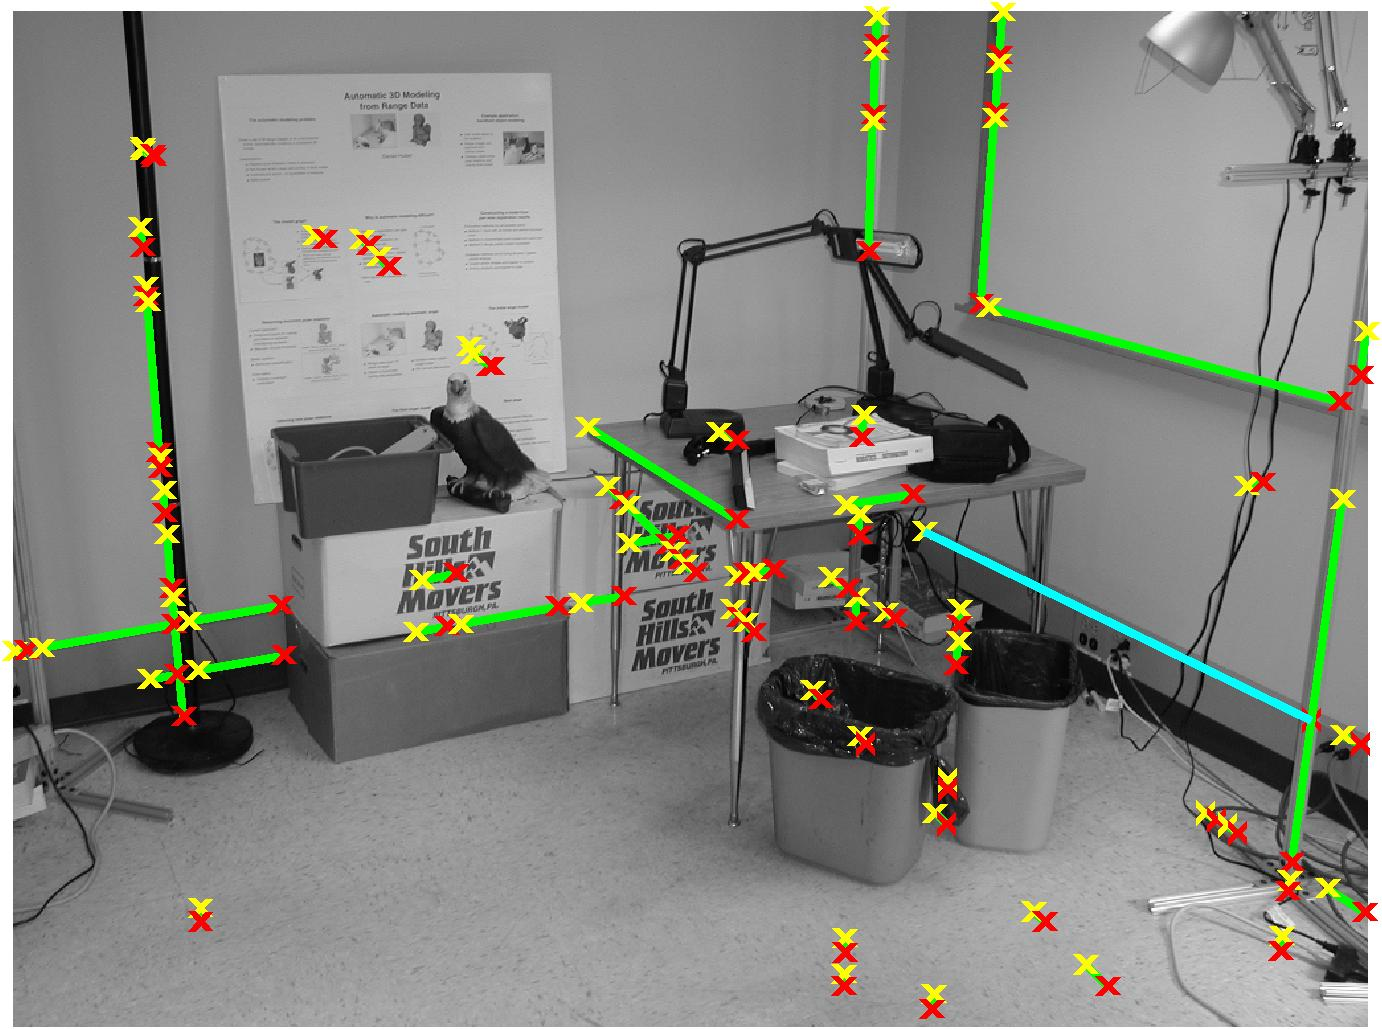
\includegraphics[width=0.8\linewidth]{hough_lines_10}
    \caption{Cluttera line segments}
    \label{fig:4}
\end{figure}

The explanation corresponds to MATLAB documentation: \emph{"houghlines(BW,theta,rho,peaks) extracts line segments in the image BW associated with particular bins in a Hough transform. theta and rho are vectors returned by function hough. peaks is a matrix returned by the houghpeaks function that contains the row and column coordinates of the Hough transform bins to use in searching for line segments."}

\subsection{Task 2}

\noindent Task 2 requires to experiment with one parameter and explain the results.

\hfill

\noindent\textbf{Quesion}: what is the effect of increasing/decreasing the required number of peaks in ‘houghpeaks’?

\hfill

\noindent\textbf{Answer}: by decresing the maximum number of peaks, only the brightest ones are marked in the \emph{Hough Map}. After extracting lines, few clear long lines can be seen (in the chosen case, 5) with few to no very short line segments. This is because at very bright peaks many sinusoids overlap, meaning many points on the same line, thus longer edge regions. By increasing the maximum number of peaks, the opposite can be observed - less bright peaks are marked in the \emph{Hough Map}, meaning there are lines made up of not as many edge points and also such lines consist of short line segments rather than being solid long lines.

\hfill

\noindent The results of the experiment on the \emph{Hough Transform} graph can be seen in \autoref{fig:5} and on the line segmentation in \autoref{fig:6}

\begin{figure}[h]
    \centering 
     
    \begin{subfigure}[h]{0.23\textwidth}
        \centering 
        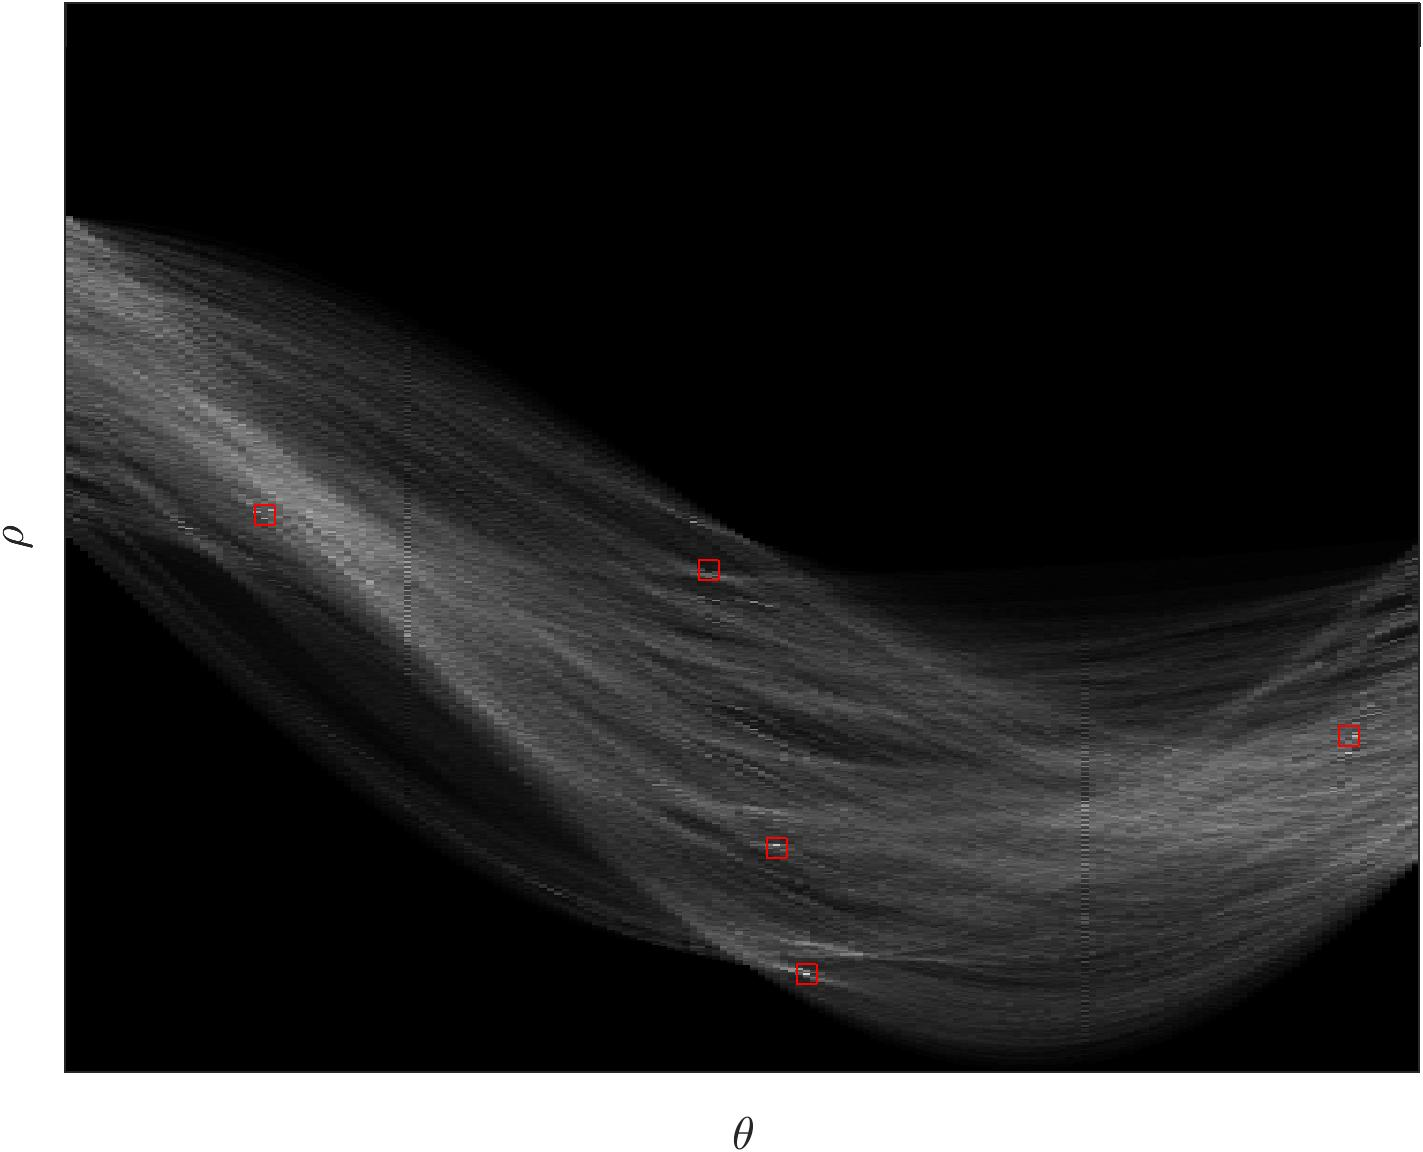
\includegraphics[width=\linewidth]{hough_transform_5}
        \caption{$\text{houghpeaks} = 5$}  
    \end{subfigure}
    % \hfill
    \begin{subfigure}[h]{0.23\textwidth}
        \centering
        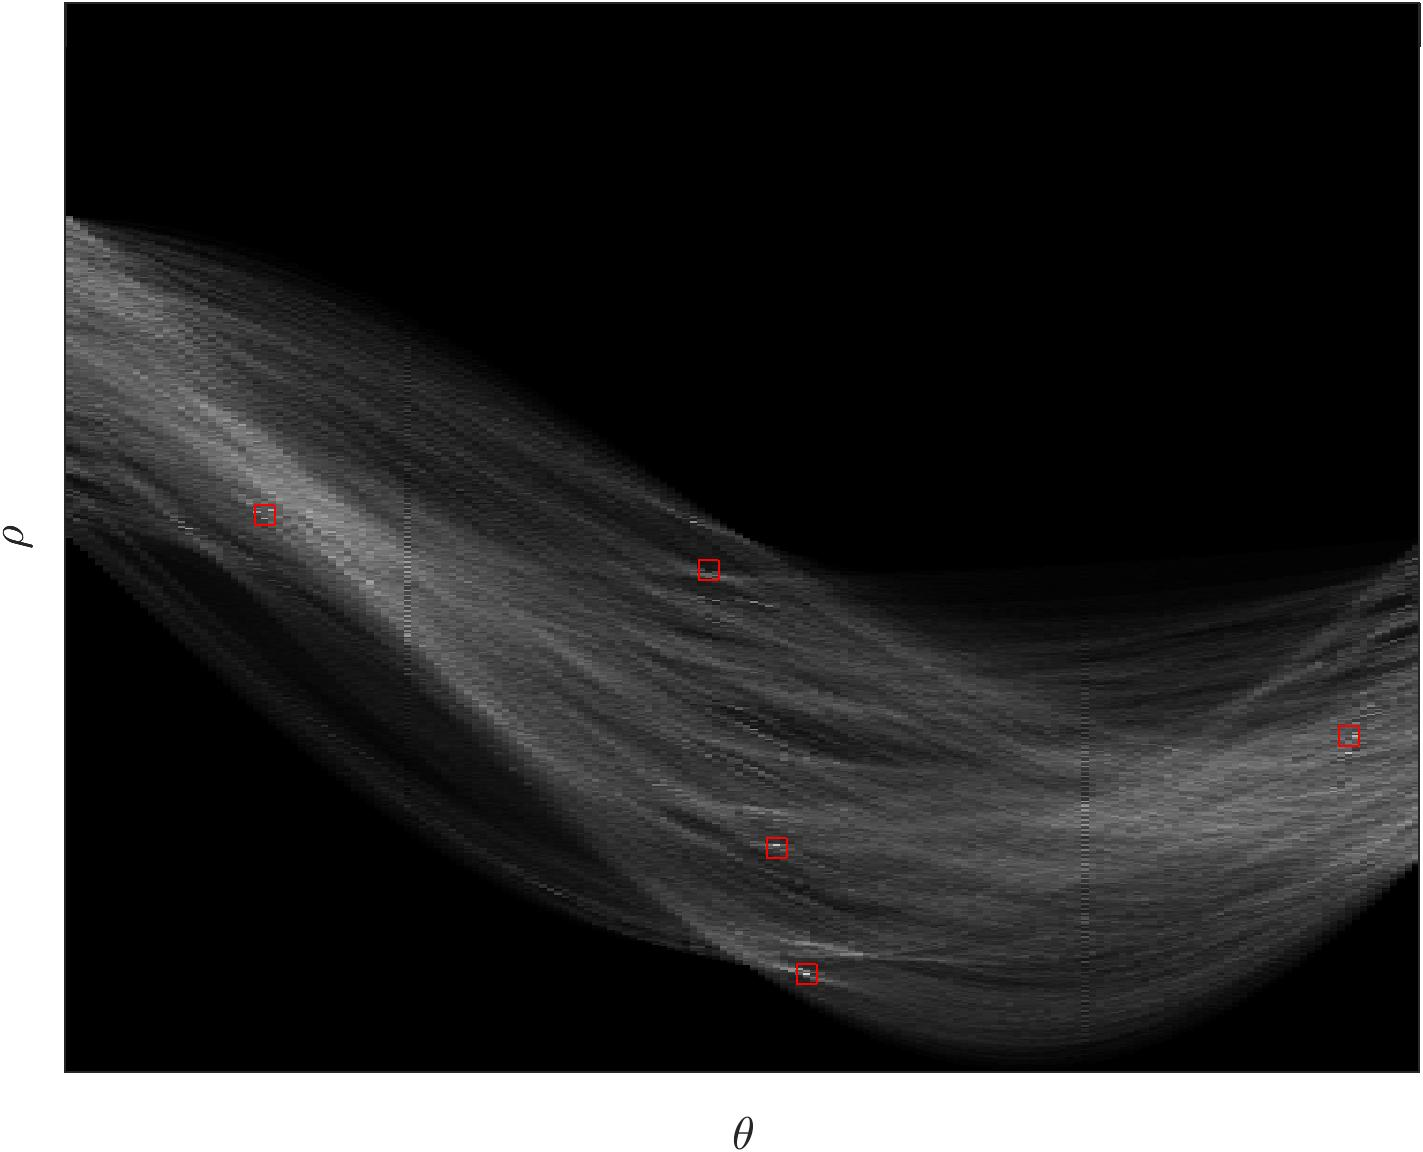
\includegraphics[width=\linewidth]{hough_transform_5}
        \caption{$\text{houghpeaks} = 20$}  
    \end{subfigure}
    % \hfill 
    \caption{Hough Transform graphs with 5 and 20 identified peaks}
    \label{fig:5}
\end{figure}

\begin{figure}[h]
    \centering 
     
    \begin{subfigure}[h]{0.23\textwidth}
        \centering 
        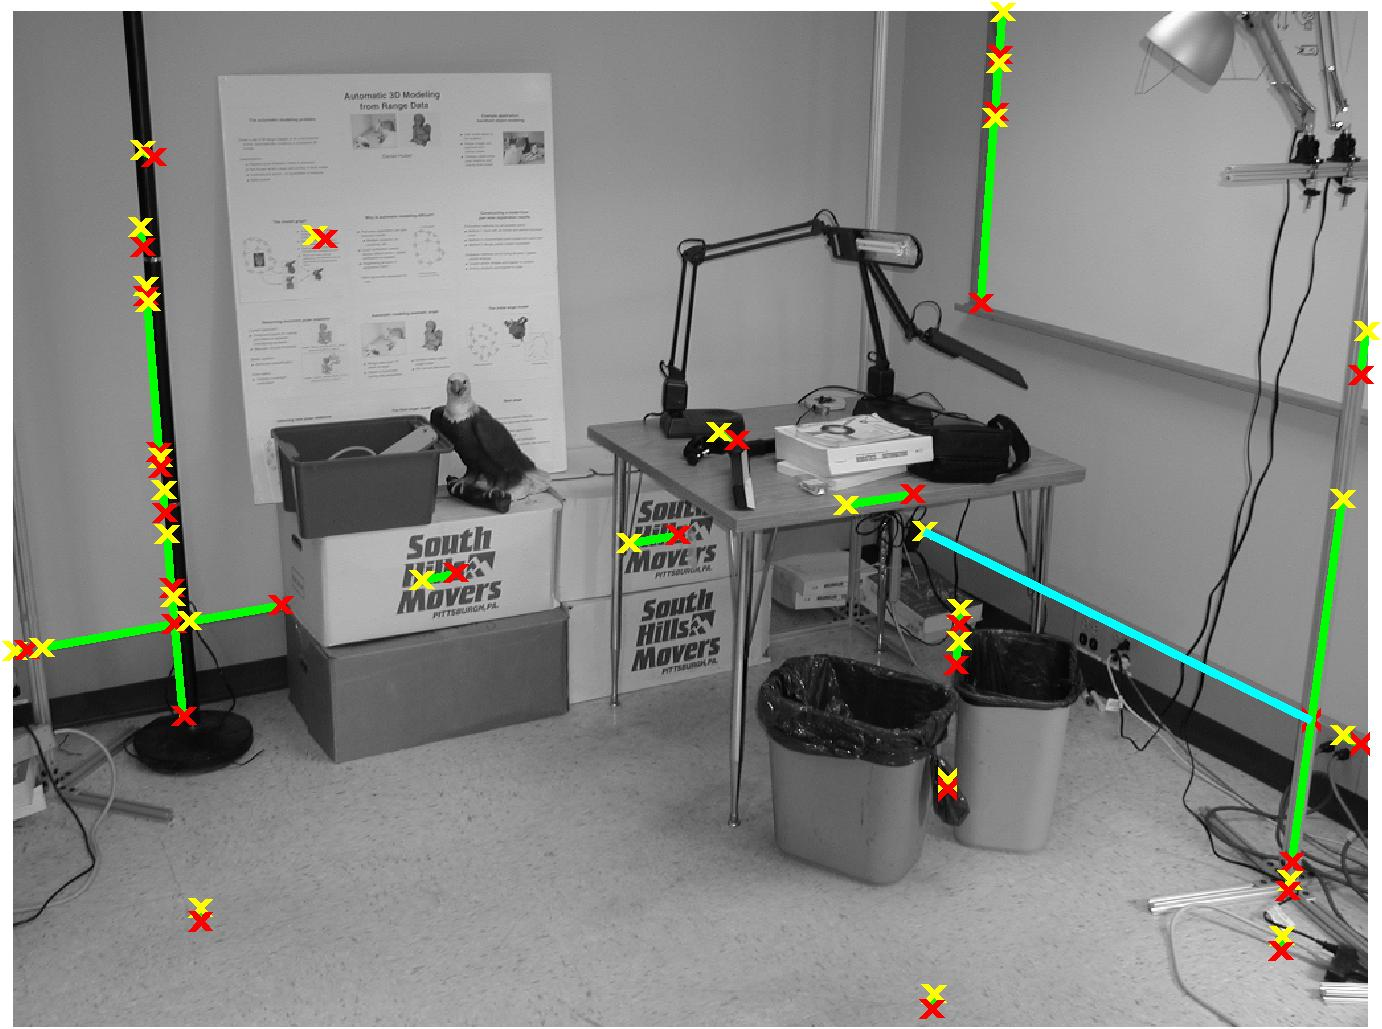
\includegraphics[width=\linewidth]{hough_lines_5}
        \caption{$\text{houghpeaks} = 5$}  
    \end{subfigure}
    % \hfill
    \begin{subfigure}[h]{0.23\textwidth}
        \centering
        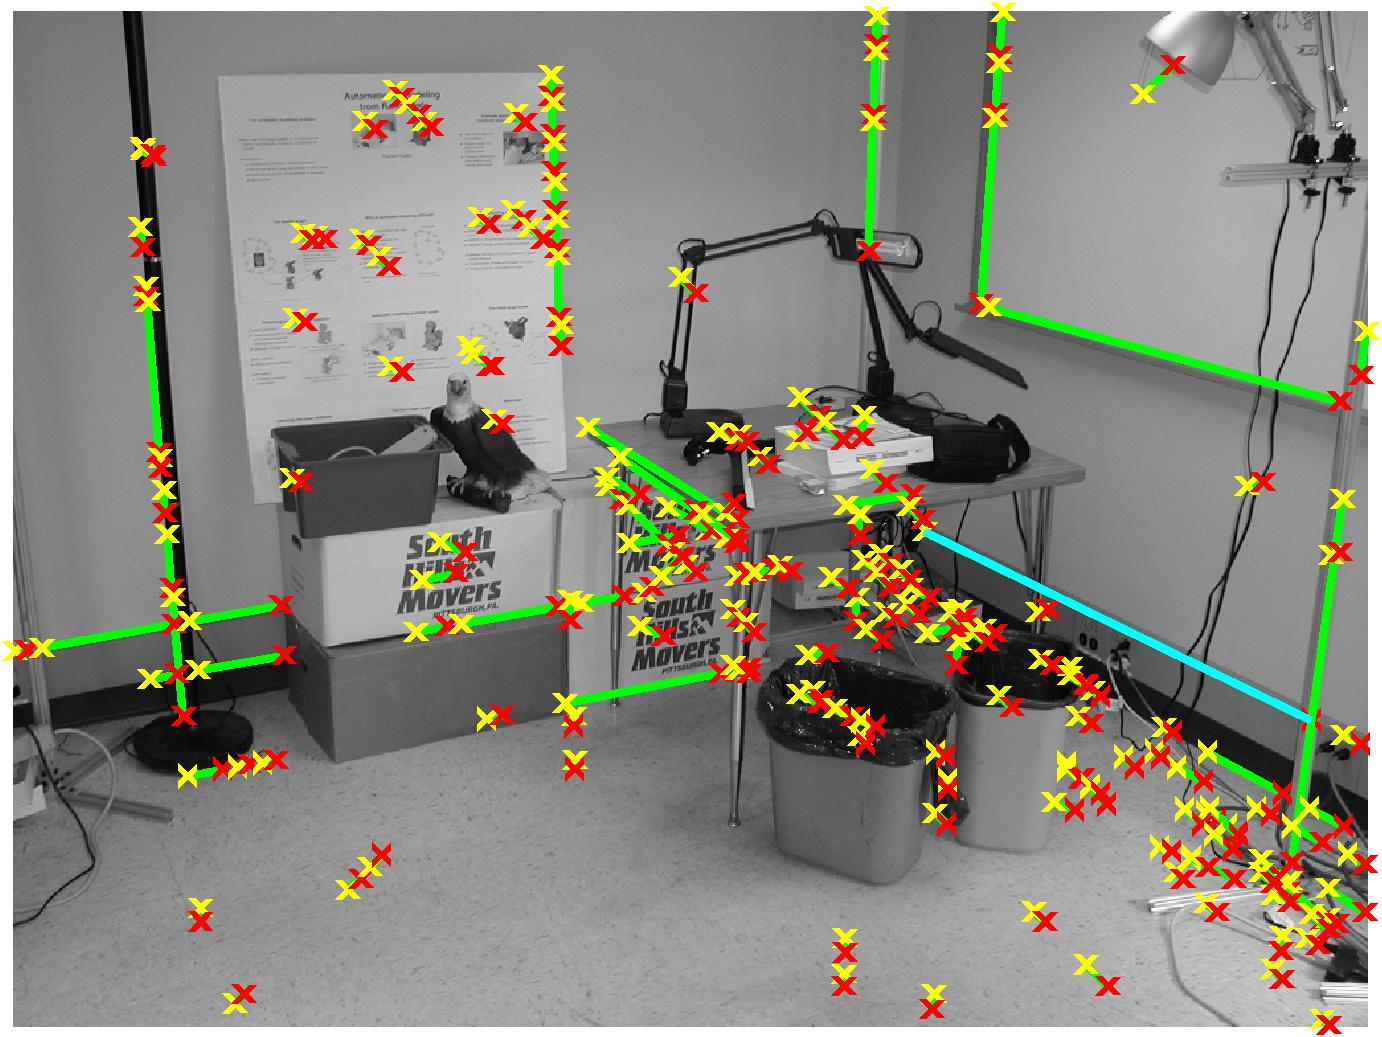
\includegraphics[width=\linewidth]{hough_lines_20}
        \caption{$\text{houghpeaks} = 20$}  
    \end{subfigure}
    % \hfill 
    \caption{Images with 5 and 20 detected major lines}
    \label{fig:6}
\end{figure}

\subsection{Task 3}

\noindent Task 3 requires to experiment with different edge detection filters to see the impact on the detected line segments.

\hfill

\noindent\textbf{Question}: replace the Canny Edge detector with other algorithms. Which one do you think performs
best and why?

\hfill

\noindent\textbf{Answer}: assuming the thresholds for each edge detection method are chosen such that they produce similar edge maps and assuming all parameters for \emph{Hough Transform} are kept the same, it seems that \emph{Canny} technique provides the best results due to its edge smoothness in the edge map, even though other filters seem to identify the specified number of lines (10 in the given case) at the same or very similar positions (note: not line segments but the general lines themselves).

\hfill

\noindent The 4 different edge maps, \emph{Hough Transform} graphs and line detection maps acquired through applying different edge detection operators can be seen in figures \ref{fig:7}, \ref{fig:8} and \ref{fig:9} respectively. The threshold chosen for \emph{Roberts} operator is $0.03$ and for both \emph{Prewitt} and \emph{Sobel} operators it is $0.025$ since filters are larger and smoothen the noise better. For \emph{Log of Gaussian} operator, \emph{zerocrossing} is applied since thresholding is not needed for 2nd order gradient map. Note that the results of the \emph{Canny} operator are not involved as they were shown previously.

\newpage

\begin{figure}[h]
    \centering 
     
    \begin{subfigure}[h]{0.21\textwidth}
        \centering 
        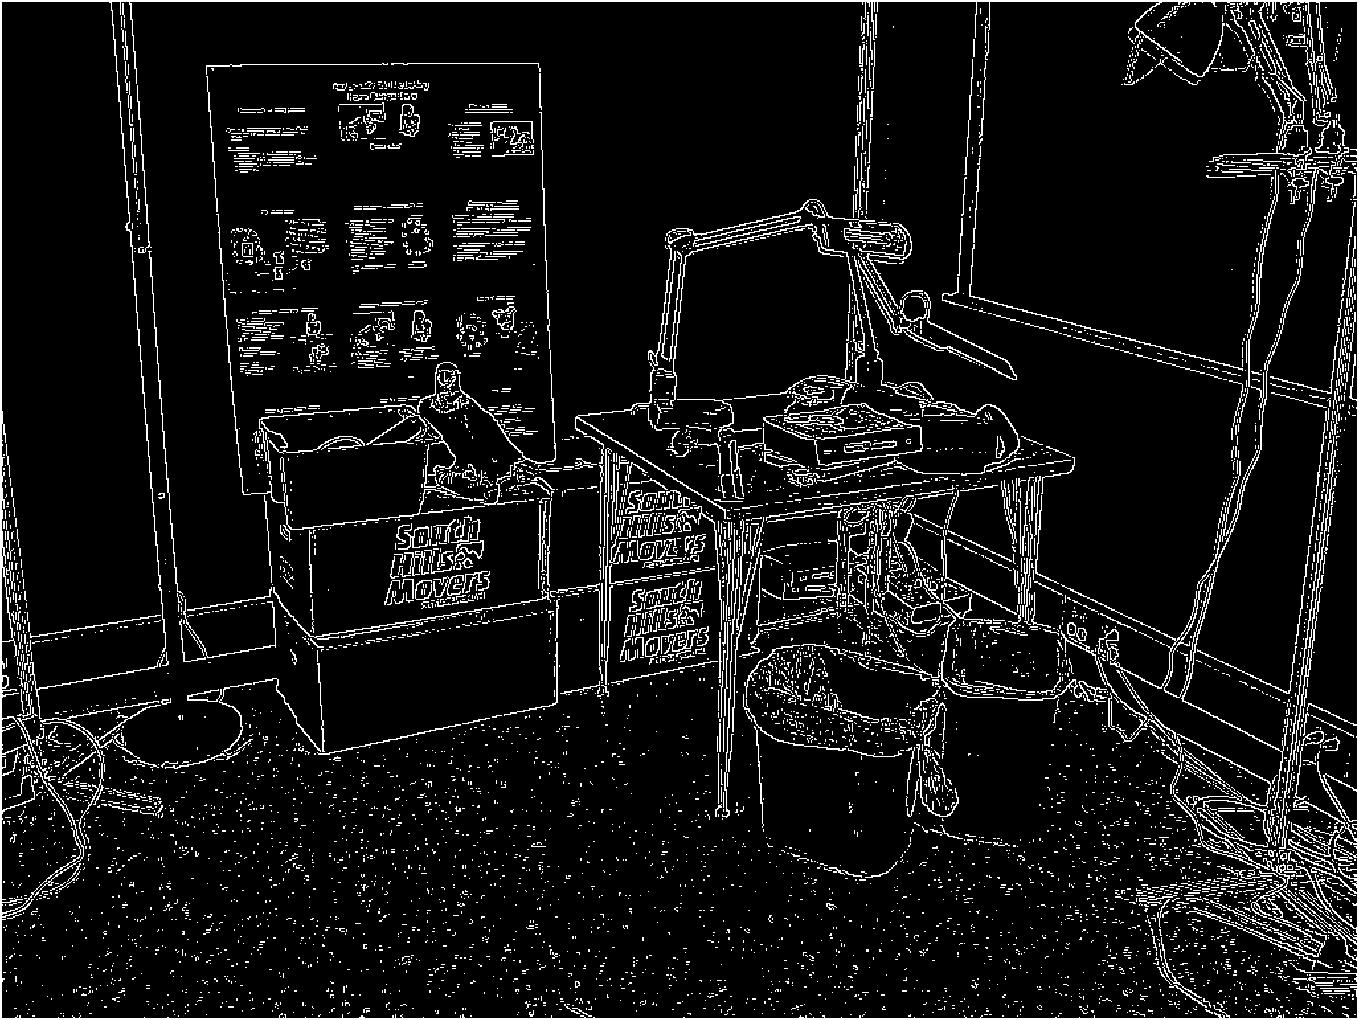
\includegraphics[width=\linewidth]{edge_map_roberts_0.03}
        \caption{Roberts}  
    \end{subfigure}
    % \hfill
    \begin{subfigure}[h]{0.21\textwidth}
        \centering
        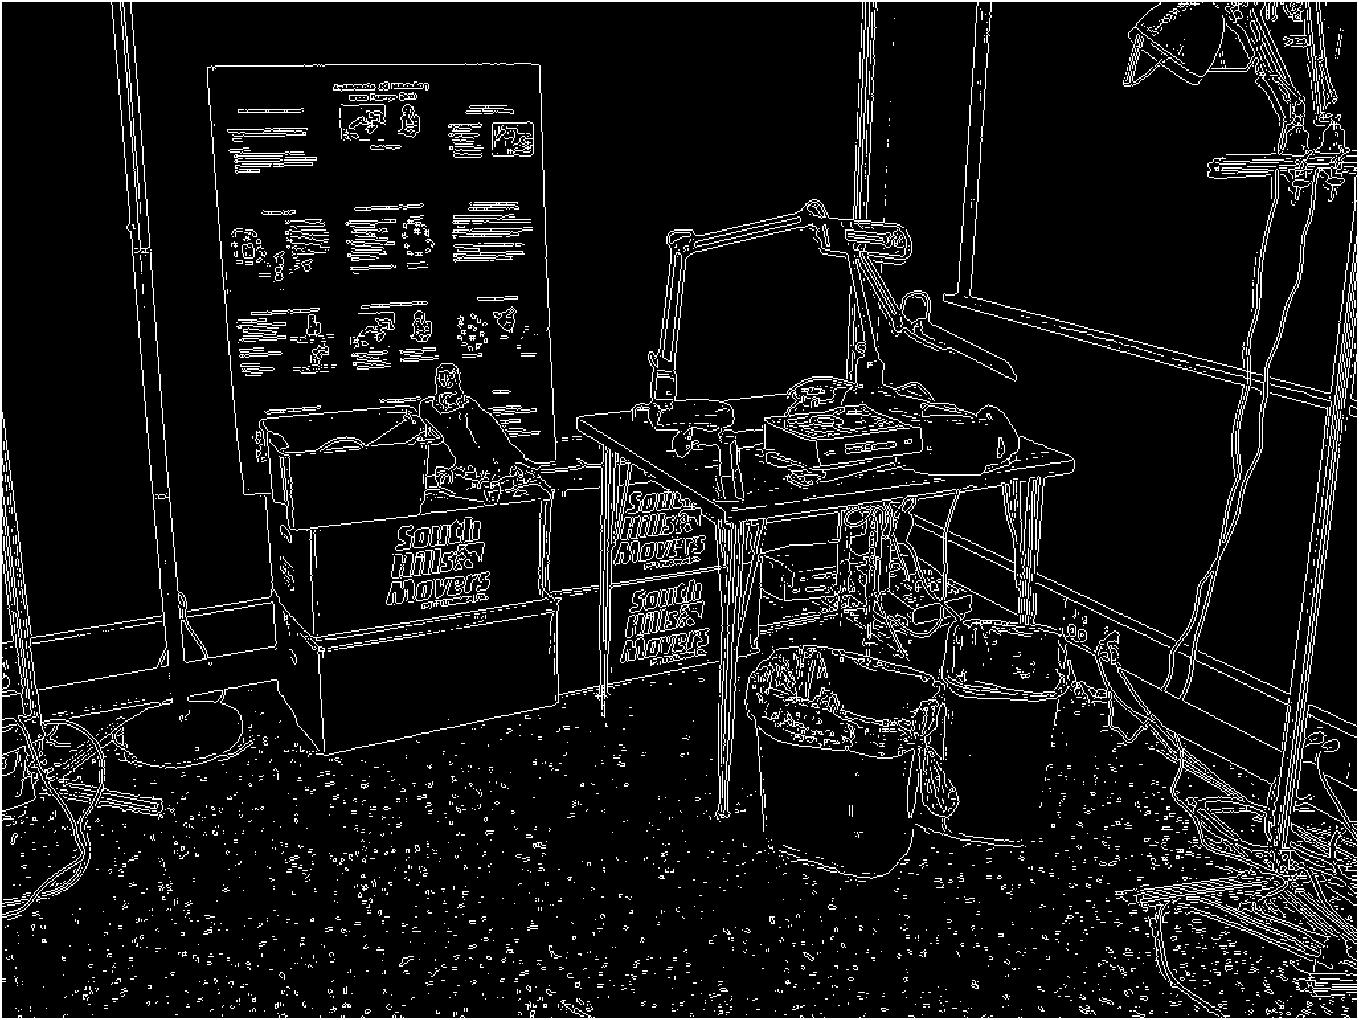
\includegraphics[width=\linewidth]{edge_map_prewitt_0.025}
        \caption{Prewitt}  
    \end{subfigure}
    % \hfill
    \begin{subfigure}[h]{0.21\textwidth}
        \centering
        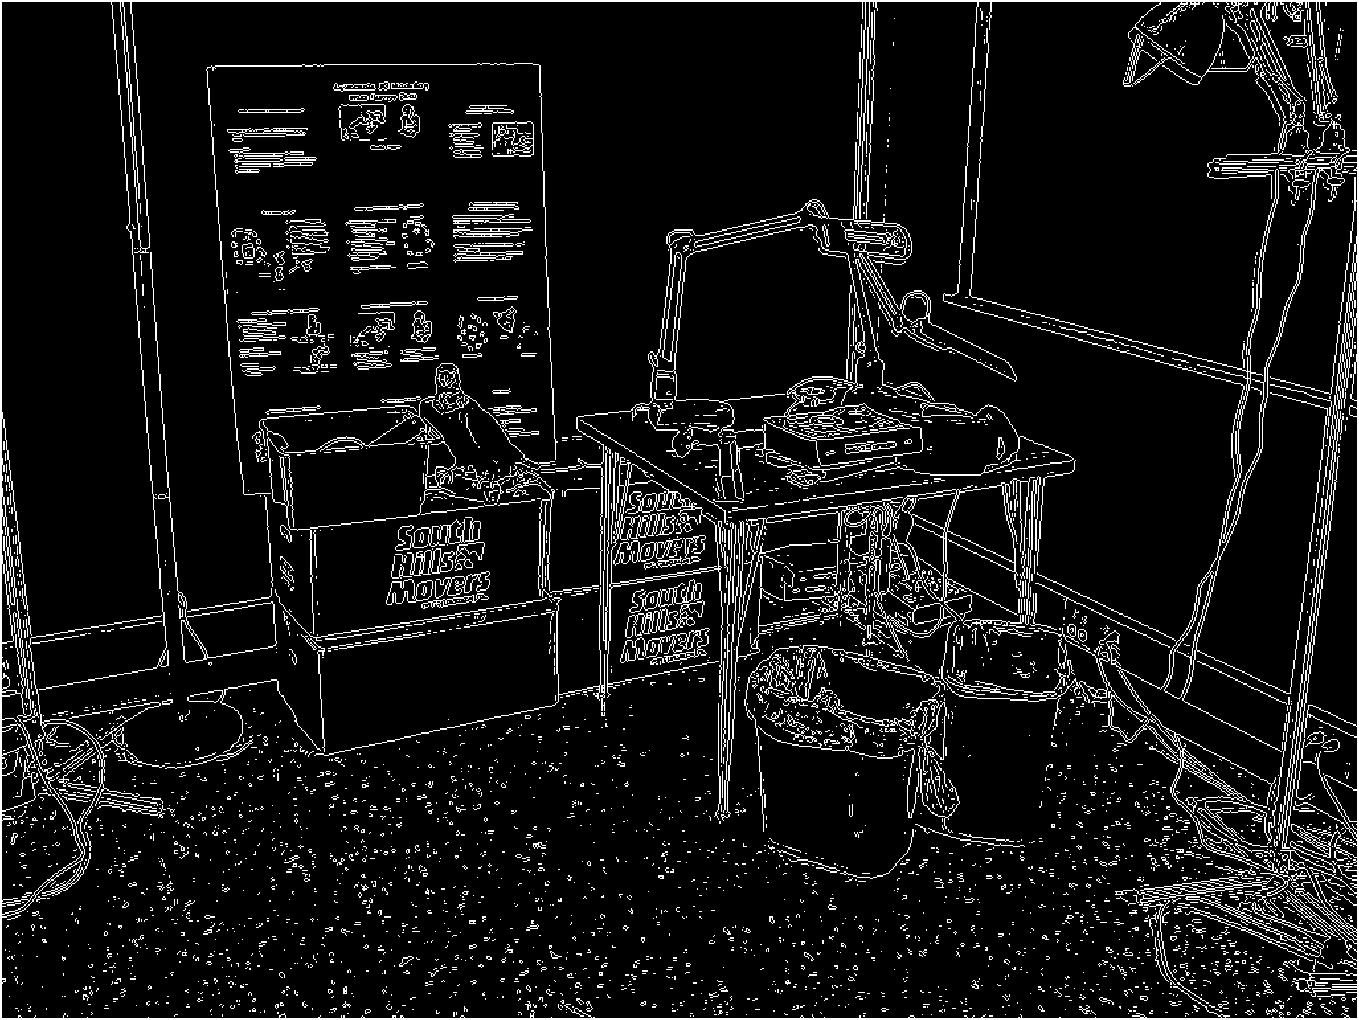
\includegraphics[width=\linewidth]{edge_map_sobel_0.025}
        \caption{Sobel}  
    \end{subfigure}
    % \hfill
    \begin{subfigure}[h]{0.21\textwidth}
        \centering
        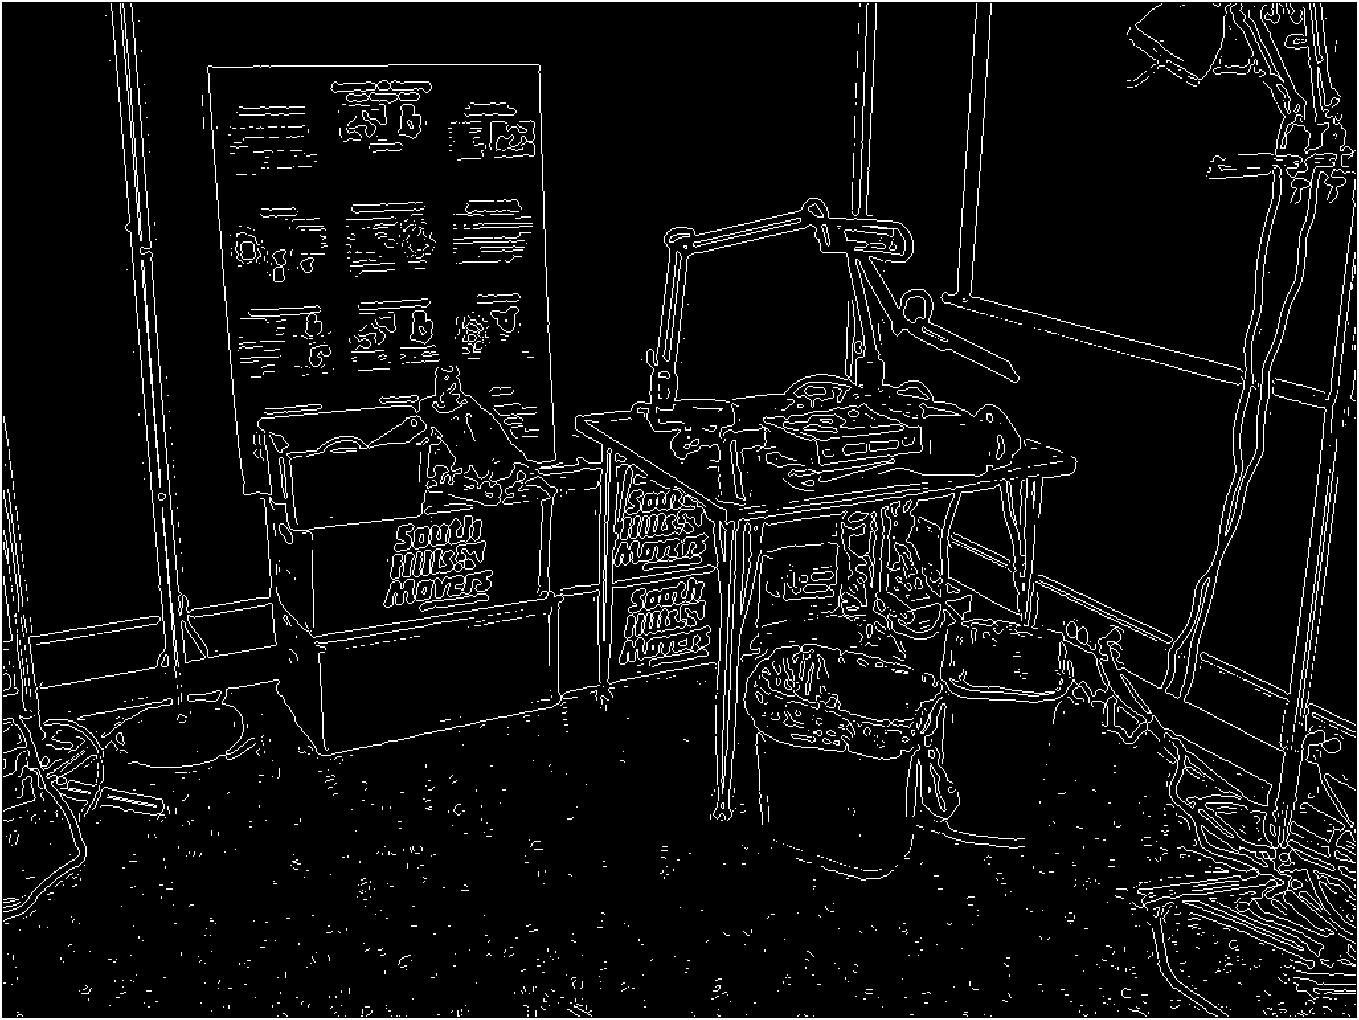
\includegraphics[width=\linewidth]{edge_map_log}
        \caption{Log of Gaussian}  
    \end{subfigure}
    % \hfill
    \caption{Edge maps by 4 different edge operators}
    \label{fig:7}
\end{figure}


\begin{figure}[h]
    \centering 
     
    \begin{subfigure}[h]{0.21\textwidth}
        \centering 
        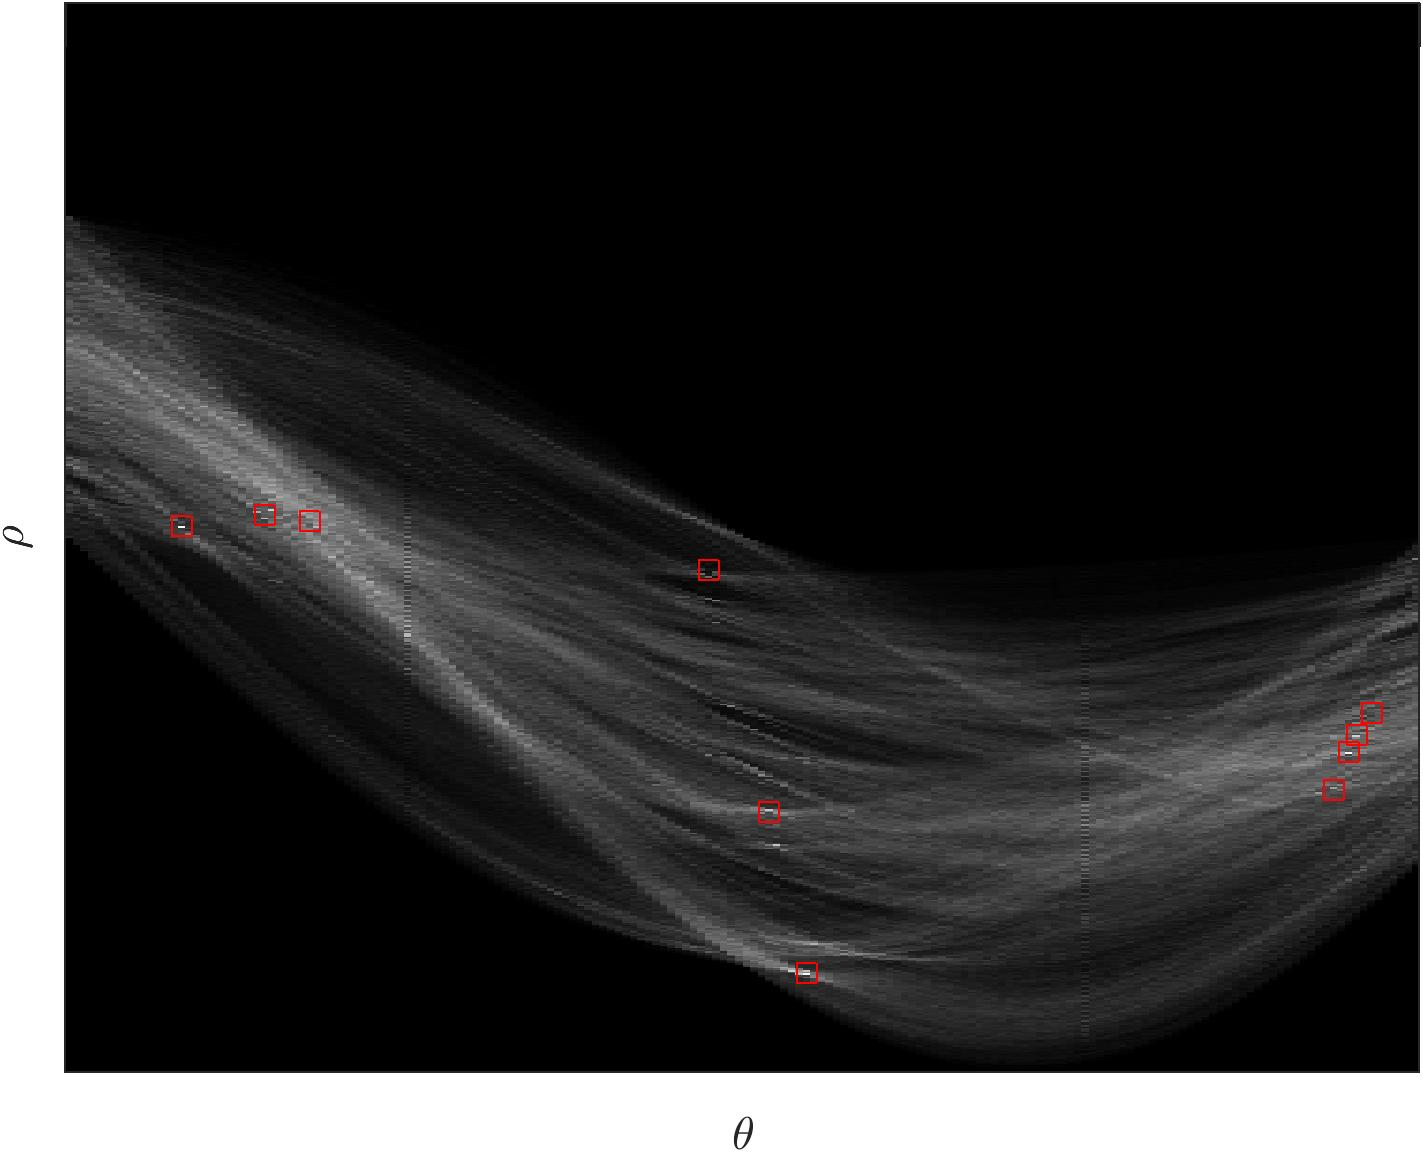
\includegraphics[width=\linewidth]{hough_transform_roberts_0.03}
        \caption{Roberts}  
    \end{subfigure}
    % \hfill
    \begin{subfigure}[h]{0.21\textwidth}
        \centering
        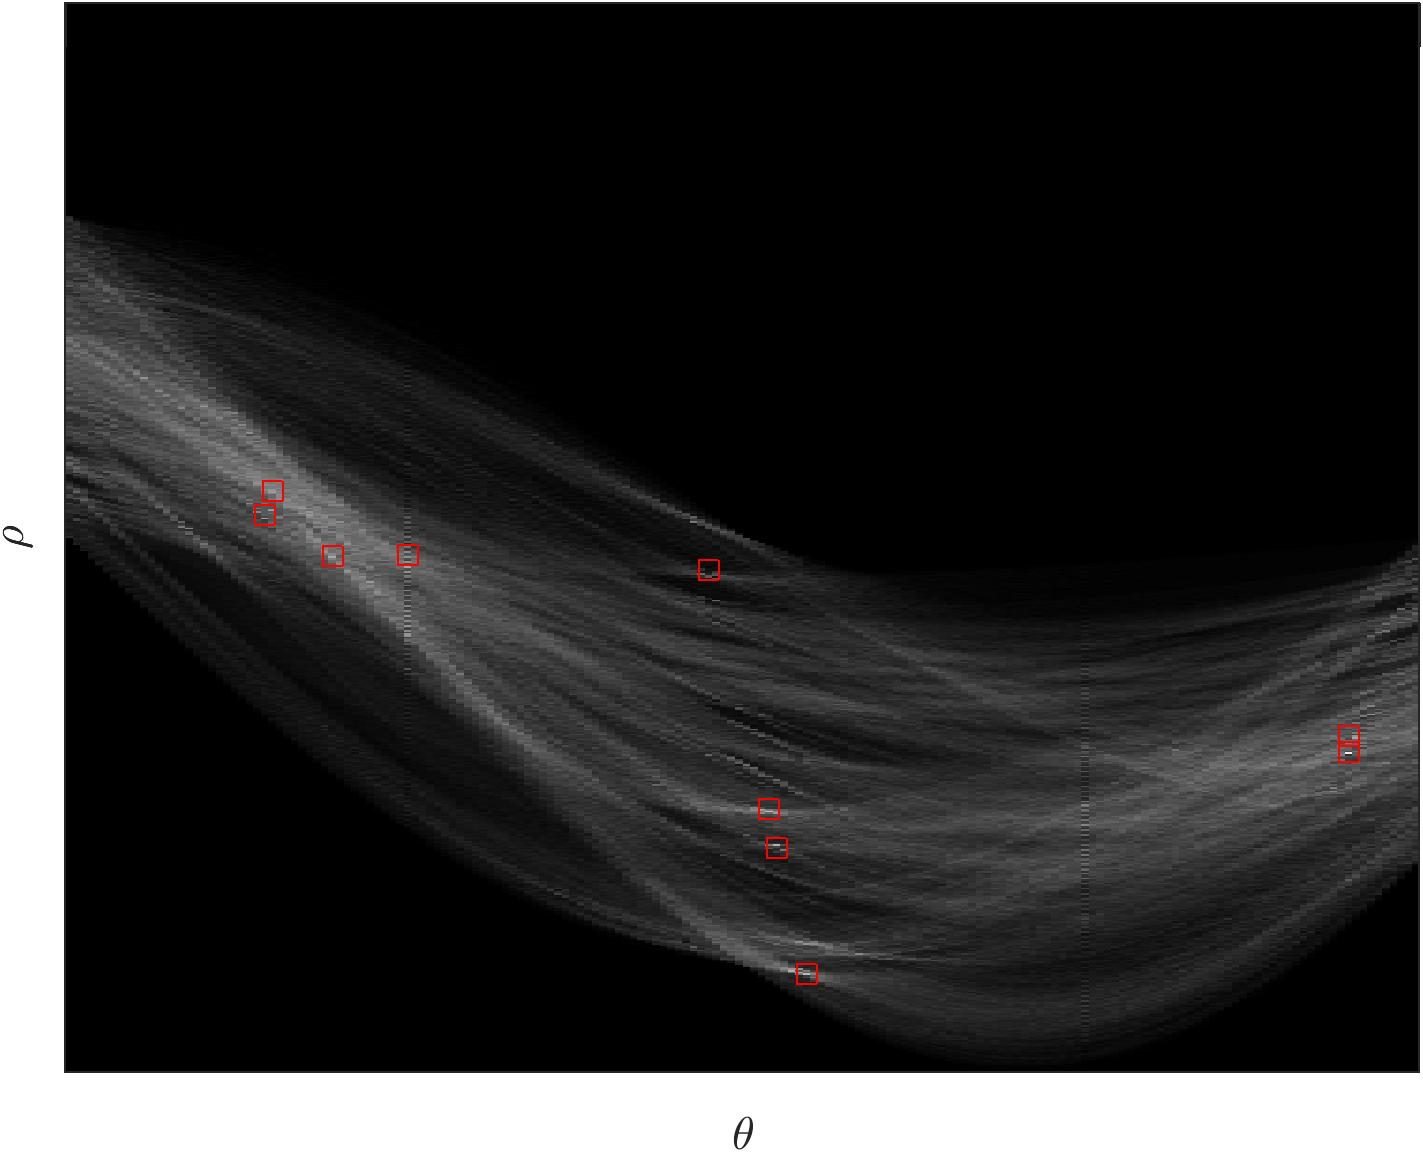
\includegraphics[width=\linewidth]{hough_transform_prewitt_0.025}
        \caption{Prewitt}  
    \end{subfigure}
    % \hfill
    \begin{subfigure}[h]{0.21\textwidth}
        \centering
        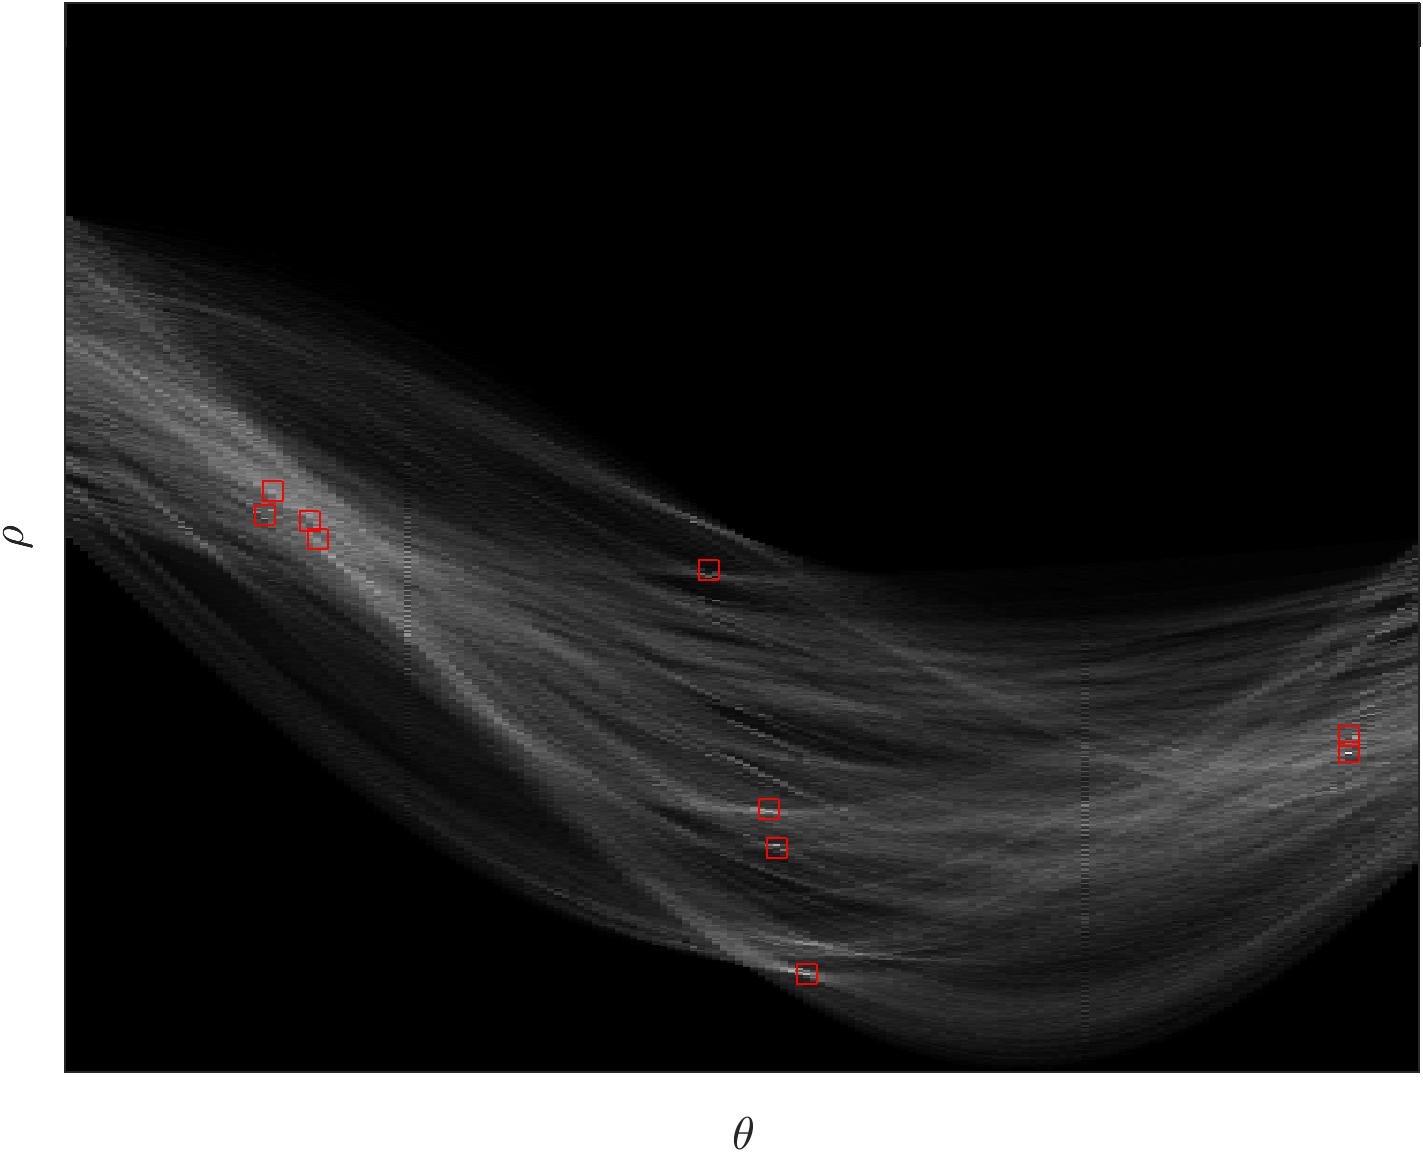
\includegraphics[width=\linewidth]{hough_transform_sobel_0.025}
        \caption{Sobel}  
    \end{subfigure}
    % \hfill
    \begin{subfigure}[h]{0.21\textwidth}
        \centering
        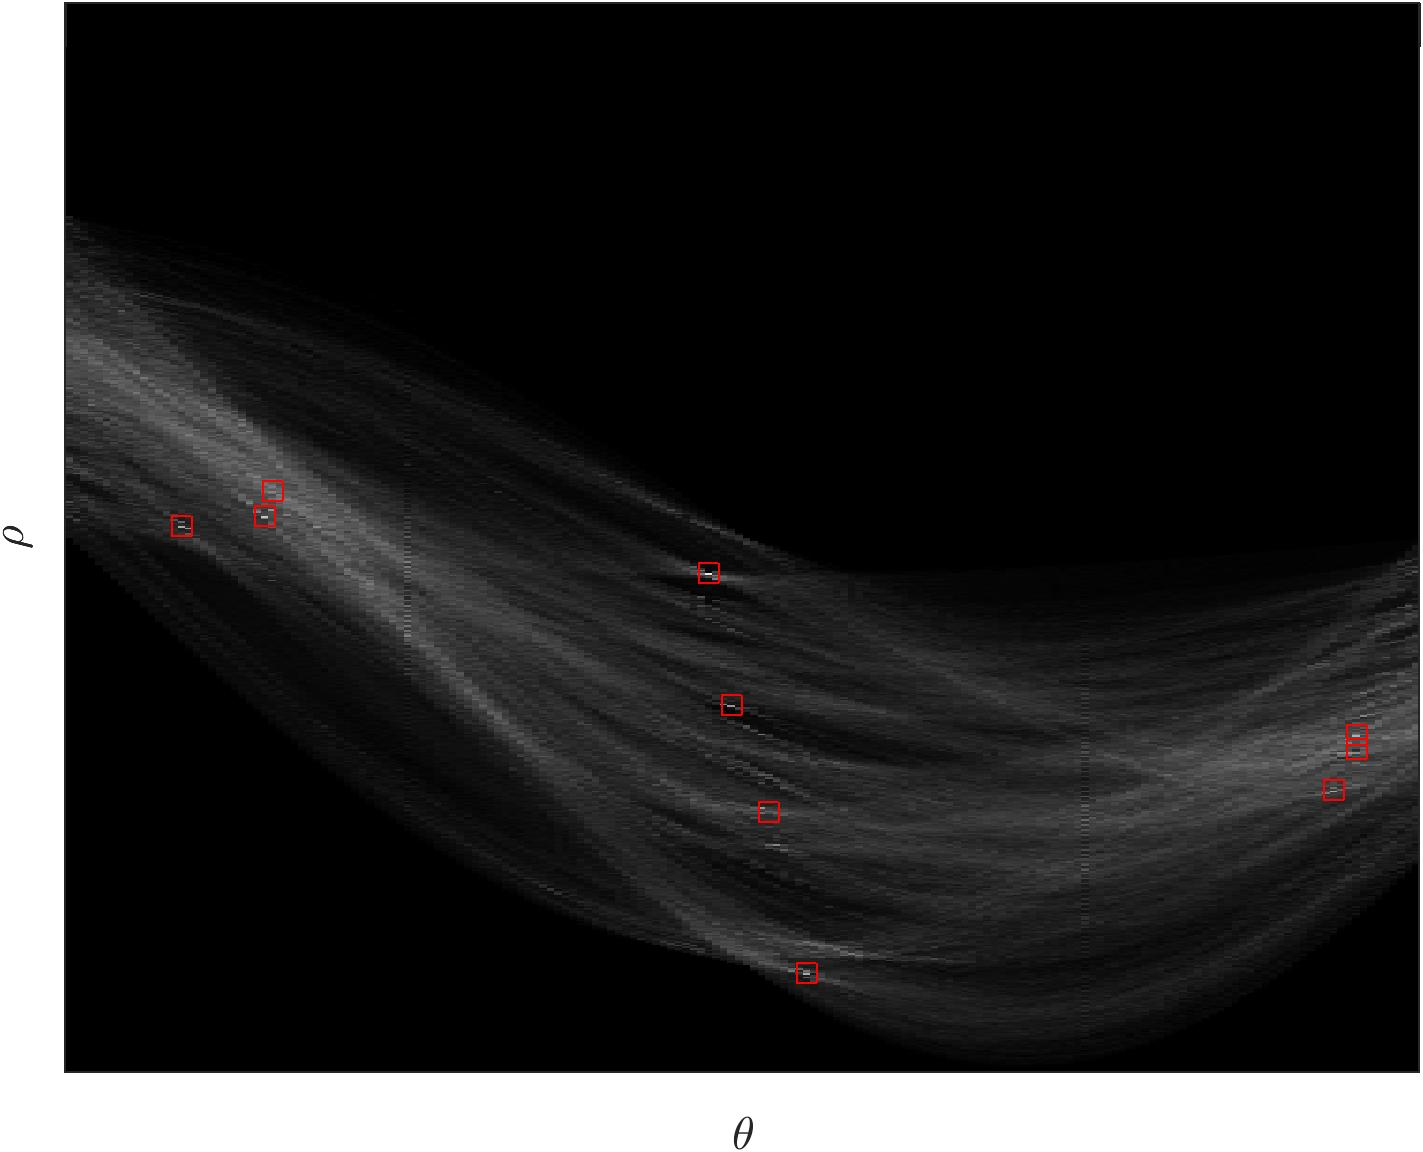
\includegraphics[width=\linewidth]{hough_transform_log}
        \caption{Log of Gaussian}  
    \end{subfigure}
    % \hfill
    \caption{Hough Transform graphs based on 4 different edge operators}
    \label{fig:8}
\end{figure}


\begin{figure}[h]
    \centering 
     
    \begin{subfigure}[h]{0.21\textwidth}
        \centering 
        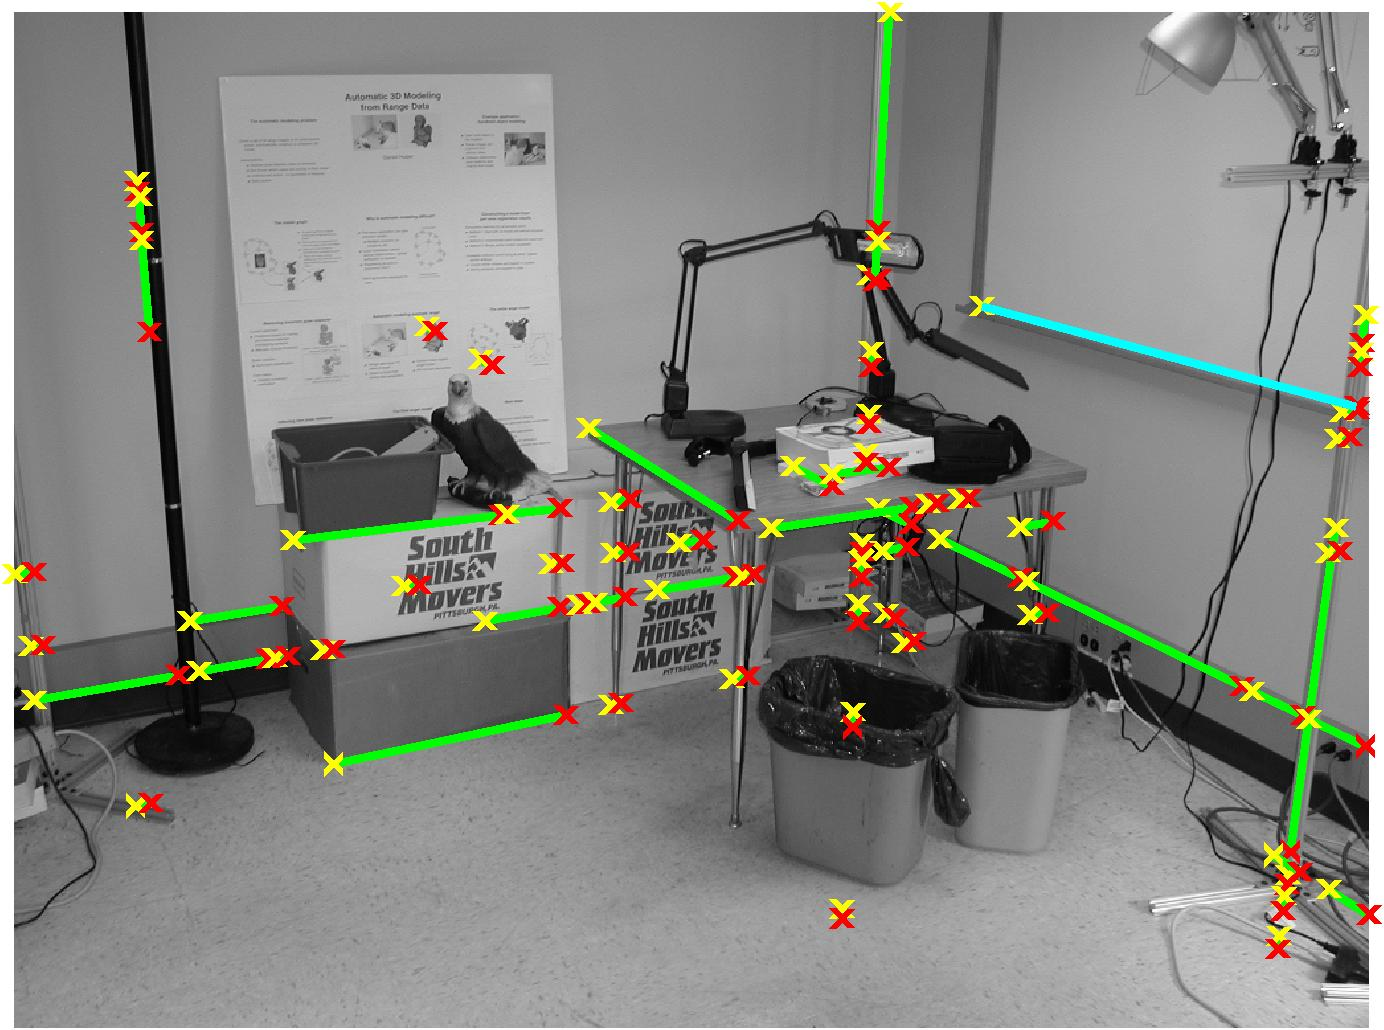
\includegraphics[width=\linewidth]{hough_lines_roberts_0.03}
        \caption{Roberts}  
    \end{subfigure}
    % \hfill
    \begin{subfigure}[h]{0.21\textwidth}
        \centering
        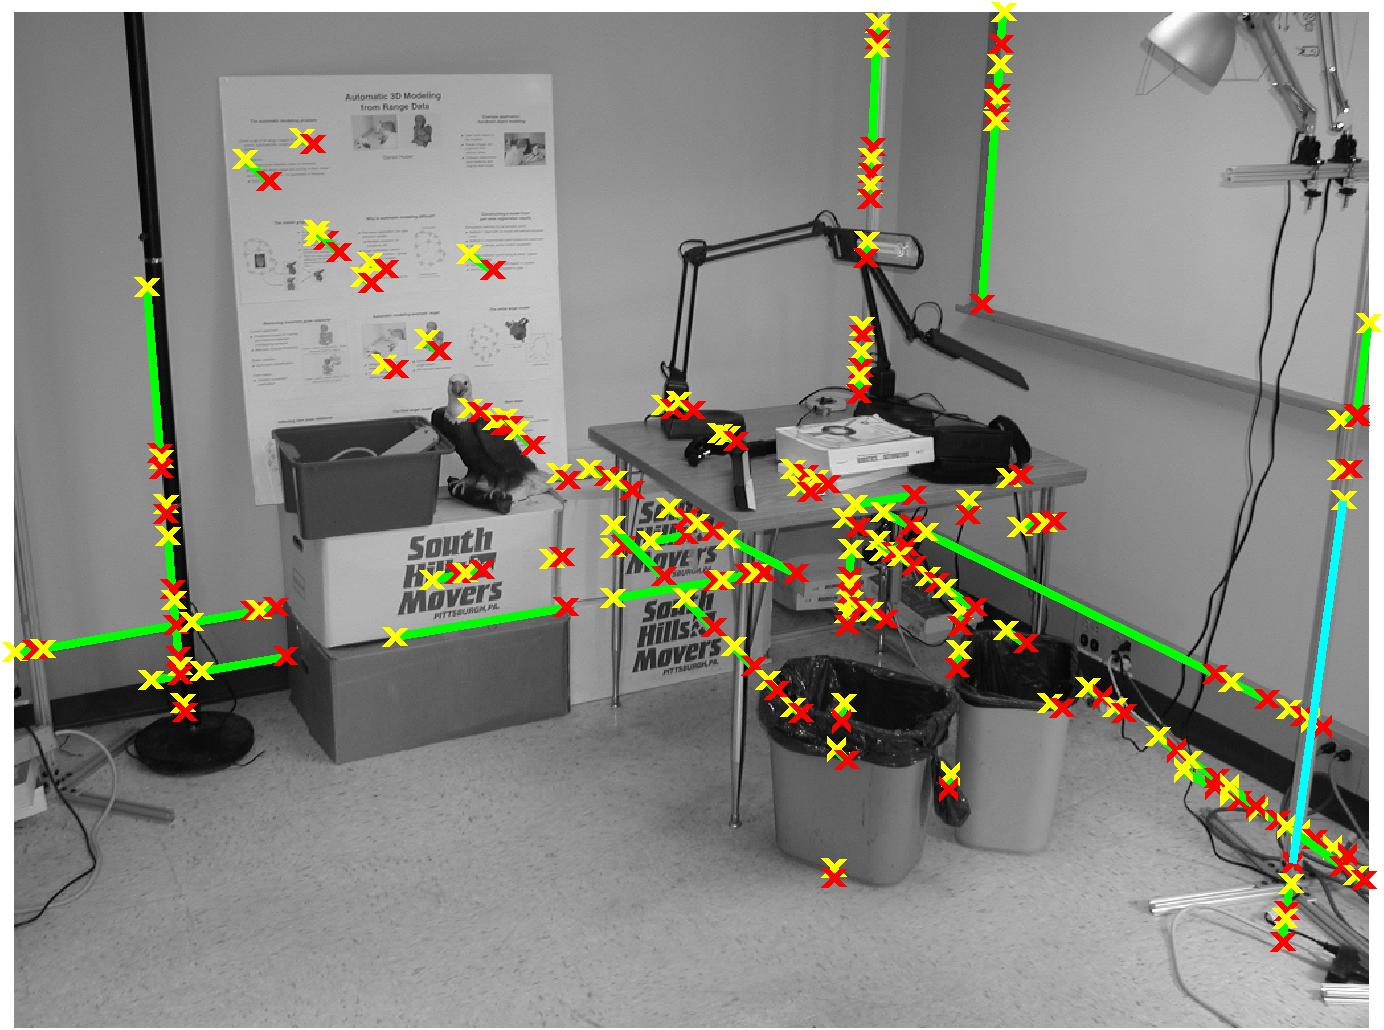
\includegraphics[width=\linewidth]{hough_lines_prewitt_0.025}
        \caption{Prewitt}  
    \end{subfigure}
    % \hfill
    \begin{subfigure}[h]{0.21\textwidth}
        \centering
        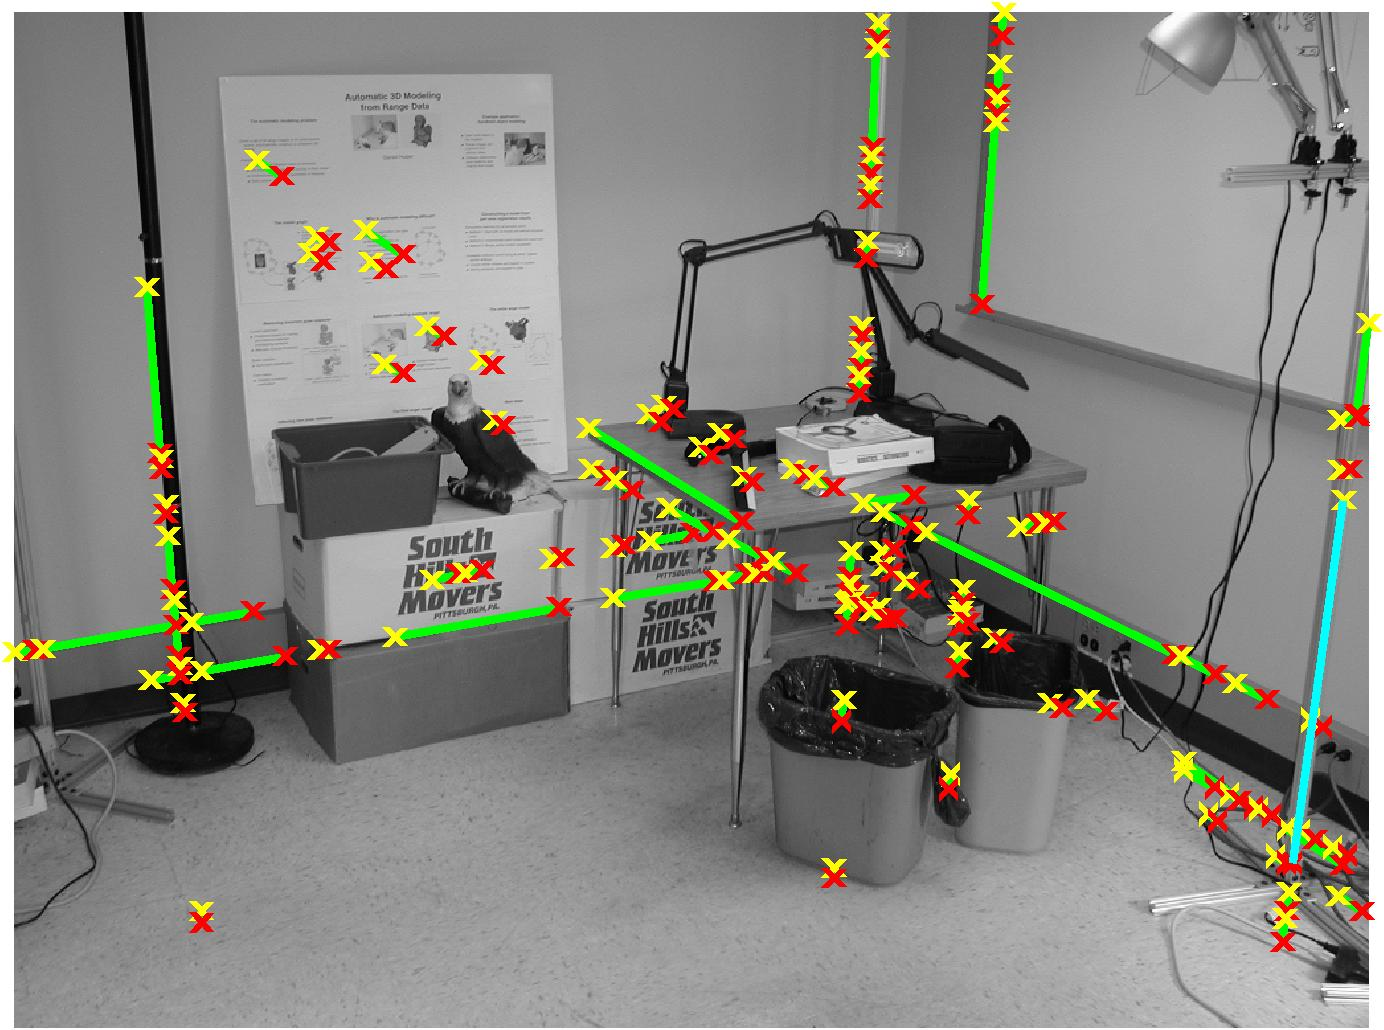
\includegraphics[width=\linewidth]{hough_lines_sobel_0.025}
        \caption{Sobel}  
    \end{subfigure}
    % \hfill
    \begin{subfigure}[h]{0.21\textwidth}
        \centering
        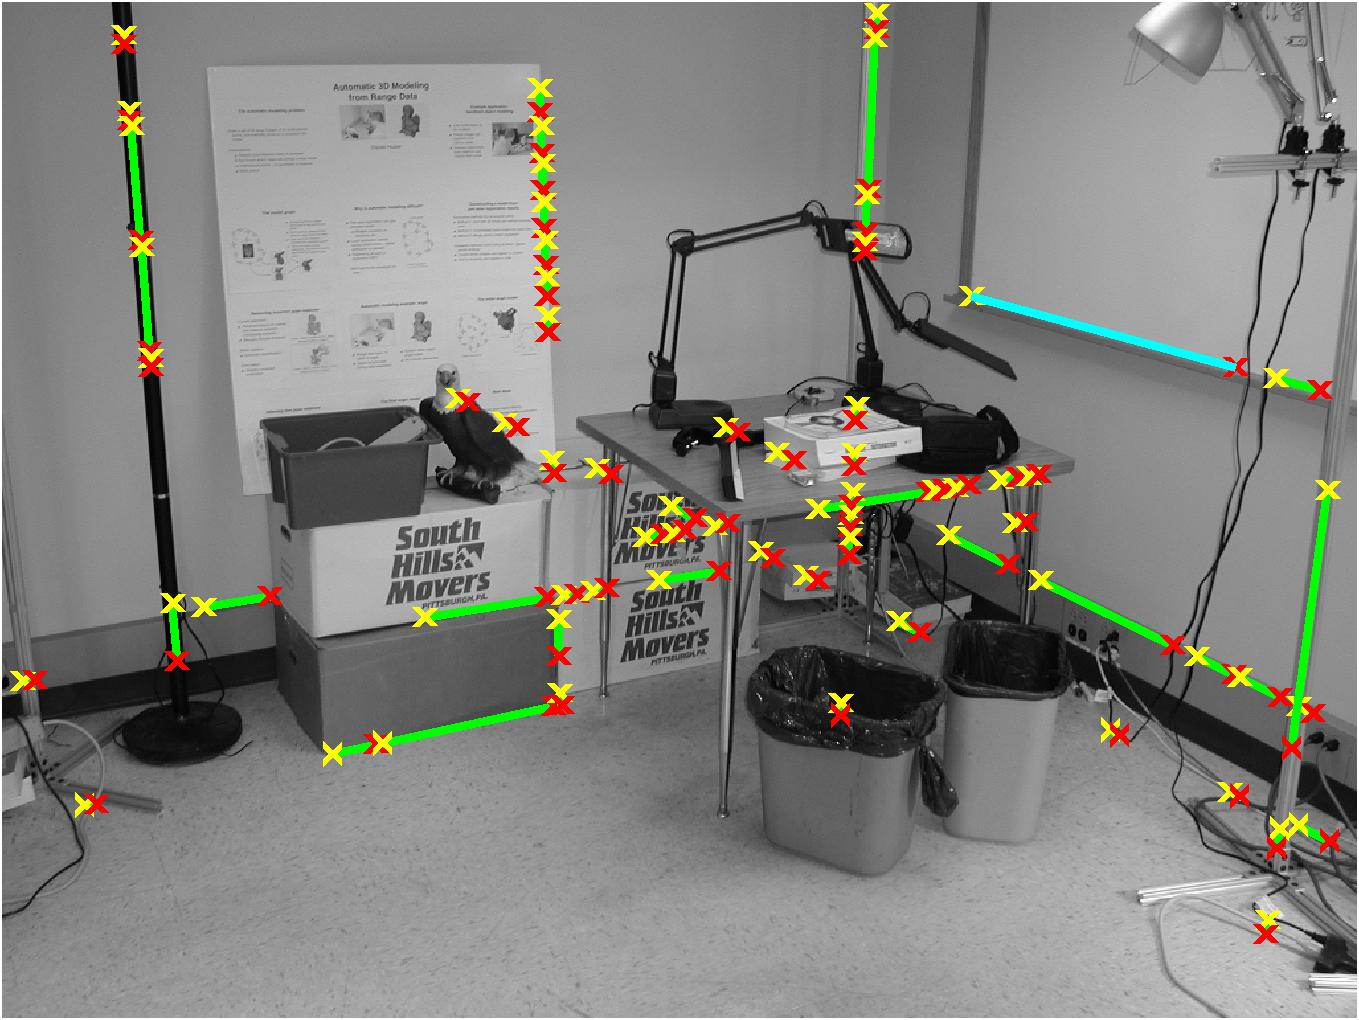
\includegraphics[width=\linewidth]{hough_lines_log}
        \caption{Log of Gaussian}  
    \end{subfigure}
    % \hfill
    \caption{Line segment maps based on 4 different edge operators}
    \label{fig:9}
\end{figure}

\noindent\textbf{Roberts} - due to a slightly higher threshold than for \emph{Prewitt} and \emph{Sobel} filters it shows less noise in the line map, i.e., it has less short line segments. Overall it captures the lines quite well, likely because it captures diagonal edges which the image possesses (boundaries are slightly tilted). It still lacks completeness for some lines, such as for the black vertical "pipe" on the left, showing that edges should be smoother for them to correspond with the line endpoints.

\hfill

\noindent\textbf{Prewitt} - because this filter is larger, a slightly lower threshold compared to \emph{Roberts} filter is enough because this filter is smoother. It still, however induces a bit more noise (due to lower threshold) meaning there are more short line segments in the line map. It is better at recognizing vertical lines than \emph{Roberts} map and generally the longest lines are longer than the longest lines when using the \emph{Roberts} filter because of more certainty in the edges.

\hfill

\noindent\textbf{Sobel} - produces very similar results to \emph{Prewitt}, however it is better because there is less noise due to larger weights in the filter on the center pixels meaning the edge map is more accurate. It has also less false line segments (segments which do not correspond to the actual edges) again because of less noise - the line detection method does not connect false positive lines simply because noise does not introduce them.

\hfill

\noindent\textbf{Laplassian of Gaussian} - this method produces great results with minimal noise. This is because the Gaussian part of the method averages the noise out and the \emph{Laplassian} part detects the edges more precisely due to the use of the 2nd order derivative. The breaking points of line segments are even more precise than when using \emph{Canny} filter. Likely, \emph{zero-crossing} points align better than thresholded points, thus giving more precise line segments. It still lacks some major lines, such as the side of the whiteboard, compared to when using \emph{Canny} - it does not have such great connectivity for weak edges (\emph{Canny} tackles that with \emph{Hysteresis thresholding}). It could potentially be a better method than \emph{Canny} if played well with \emph{Hough} line detection parameters.


\begin{thebibliography}{1}
\bibliographystyle{IEEEtran}

\bibitem{ref1}
Canny, John, "A Computational Approach to Edge Detection," {\it{IEEE Transactions on Pattern Analysis and Machine Intelligence}}, Vol. PAMI-8, No. 6, 1986, pp. 679-698

\bibitem{ref2}
Rafael C. Gonzalez, Richard E. Woods, Steven L. Eddins, "Digital Image Processing Using MATLAB", 2nd ed., Gatesmark Publishing, 2009

\bibitem{ref3}
Rafael C. Gonzalez, Richard E. Woods, Steven L. Eddins, "Digital Image Processing Using MATLAB", Prentice Hall, 2004

\bibitem{ref4}
Rafael C. Gonzalez, Richard E. Woods, Steven L. Eddins, "Digital Image Processing Using MATLAB", Prentice Hall, 2003

\end{thebibliography}

\end{document}